\documentclass[12pt, a4paper]{article}
\usepackage[margin=0.8in]{geometry}
\usepackage[utf8]{inputenc}
\usepackage{hyperref}
\usepackage{graphicx}
\usepackage{caption}
\usepackage{amsmath,amsfonts,amssymb,empheq}
\usepackage{bm}
\usepackage[dvipsnames]{xcolor}

\setlength{\parskip}{5pt}

\title{Solved Problems on \\ Control of Nonlinear Spacecraft Attitude Motion}
\author{by \\ Rishav}
\date{May 2021}

\newcommand{\ans}{\item[]$\rlap{\LARGE{\checkmark}}\square\quad$}
\newcommand{\noans}{\item[]$\square\quad$}

\begin{document}

\maketitle
\tableofcontents

\newpage
\section{Week 1 - Nonlinear Stability Definitions}
\subsection{State Vector Representation}
\paragraph{1.}
$\ddot{x} + \sin(x) = 0$, what is the first order state-space representation? What is a proper state vector of this system?

\begin{itemize}
\noans $\text{\bf{x}} = (x_{1})$ with $x_{1} = x$
\ans  $\text{\bf{x}} = (x_{1},x_{2})$ with $x_{1} = x$, $x_{2} = \dot{x}$
\noans  $\text{\bf{x}} = (x_{1},x_{2},x_{3})$ with $x_{1} = x$, $x_{2} = \dot{x}$, $x_{3} = \ddot{x}$
\end{itemize}

\paragraph{\textcolor{orange}{Solution:}} 
Dynamical system described by $n^\text{th}$ order differential equation has state vector $\text{\bf{x}} \in \mathbb{R}^{n}$.

\paragraph{2.}
What is an equivalent state-space representation for Question 1?

\begin{itemize}
\noans $\dot{x}_{1} = -\sin(x_{1})$
\noans $\begin{bmatrix} \dot{x}_{1} \\ \dot{x_{2}}\end{bmatrix} = \begin{bmatrix} \sin(x_{1}) \\ x_{2}\end{bmatrix}$
\ans $\begin{bmatrix} \dot{x}_{1} \\ \dot{x_{2}}\end{bmatrix} = \begin{bmatrix} x_{2} \\ -\sin(x_{1}) \end{bmatrix}$
\end{itemize}

\paragraph{\textcolor{orange}{Solution:}} 
State-space representation describes the given second-order differential equation as the set of two first-order coupled differential equations. Let $x_{1} = x$ and $x_{2} = \dot{x}$, then we have:

\begin{equation*}
\begin{split}
\text{First equation}&: \dot{x}_{1} = \dot{x}\\
\text{Second equation}&: \ddot{x} = \dot{x}_{2} = -\sin(x_{1}) \\
\end{split}
\end{equation*}

\paragraph{3.}
For a mechanical dynamical system with $N$ degrees of freedom, what is the minimal dimension of the corresponding state vector?

\begin{itemize}
\noans $N$
\ans $2N$
\noans $\cfrac{N(N-1)}{2}$
\end{itemize}

\paragraph{\textcolor{orange}{Solution:}}
The concept of the \textit{state} of a dynamic system refers to at least a minimum set of variables, known as \textit{state variables}, that fully describe the system and its response to any given set of inputs. The dimension of the state vector is at least twice the \textit{degrees of freedom} of that system.

\paragraph{4.}
What are the equilibrium states of $\ddot{x} + \sin(x) = 0$?

\begin{itemize}
\noans $x=0$
\noans $x=\pi$
\ans $x=n\pi$ where $n$ is any integer number
\end{itemize}

\paragraph{\textcolor{orange}{Solution:}}
A state vector point $\bm{x}_{e}$ is said to be an equilibrium state (or equilibrium point) of a dynamical system described by $\dot{\bm{x}} = \bm{f}(\bm{x},\bm{u})$ at time $t_{o}$ if
$$\dot{\bm{x}} = \bm{f}(\bm{x}_{e},\bm{u}) = 0 \quad \quad \forall t > t_{o}$$

State-space representation of $\ddot{x} + \sin{x} = 0$ with state vector $\text{\bf{x}} = [x_{1}\;x_{2}]^{\intercal}$ is
$$\dot{\text{\bf{x}}} = \begin{bmatrix} \dot{x}_{1} \\ \dot{x_{2}}\end{bmatrix} = \begin{bmatrix} x_{2} \\ -\sin(x_{1})\end{bmatrix} \text{ where, } x_{1} = x \text{ and } x_{2} = \dot{x}_{1}$$

We need value of $x$ for which $\dot{\text{\bf{x}}} = 0$ (i.e. $\dot{x} = 0$ and $-\sin(x) = 0$).$-\sin(x) = 0$ implies $x = n\pi$ where $n$ is a integer.

\paragraph{5.}
What are the equilibrium states of $\ddot{x} + x - x^3 = 0$?

\begin{itemize}
\ans $x_{\epsilon} \in \{0,\pm 1\}$
\noans $x_{\epsilon} = 0$
\noans $x_{\epsilon} = \pm 1$
\end{itemize}

\paragraph{\textcolor{orange}{Solution:}}
State-space representation of $\ddot{x} + x - x^3 = 0$ with state vector $\text{\bf{x}} = [x_{1}\;x_{2}]^{\intercal}$ is
$$\dot{\text{\bf{x}}} = \begin{bmatrix} \dot{x}_{1} \\ \dot{x_{2}}\end{bmatrix} = \begin{bmatrix} x_{2} \\ x_{1}^{3}-x_{1} \end{bmatrix} \text{ where, } x_{1} = x \text{ and } x_{2} = \dot{x}_{1}$$

 
We need value of $x$ for which $\dot{\text{\bf{x}}} = 0$ (i.e. $\dot{x} = 0$ and $x^{3}-x = 0$). $x^{3}-x = 0$ implies $x = \{0,\pm1\}$.


\newpage
\subsection{State Neighborhood}
\paragraph{1.}
If $\bm{x} = (1,2,3)$, is $\bm{x} \in B_{1}(\bm{0})$?

\begin{itemize}
\noans The states contain 1, thus this is true
\noans There is not enough information to say
\ans No, the $L_{2}$ norm of $\bm{x}$ is about 3.74, which is outside the unit Ball centered around $(0,0,0)$
\end{itemize}

\paragraph{\textcolor{orange}{Solution:}}
Given $\delta > 0$, a state vector $\bm{x}(t)$ is said to be in the neighborhood $\bm{B}_{\delta}(\bm{x}_{r}(t))$ of the state $\bm{x}_{r}(t)$ if
$$|\!|\bm{x}(t) - \bm{x}_{r}(t)|\!| < \delta \implies \bm{x}(t) \in \bm{x}_{r}(t)$$
where, $|\!|\,|\!|$ is $L_{2}$ norm. \medskip

In this problem, $\bm{x}=(1,2,3)$, $\bm{x}_{r} = (0,0,0)$ and $\delta = 1$ so, $\bm{x} \in B_{1}(\bm{0})$ if $|\!|\bm{x} - \bm{0}|\!| < 1$ which is not true.

\paragraph{2.}
Let a particle position be defined by $\bm{r} = (\sin(t), \cos(t), 0)$ where $\bm{t}$ is time. What is a neighborhood that will contain this motion?

\begin{itemize}
\ans $B_{1.1}(\bm{x}_{r} = (0,0,0))$
\noans $B_{1}(\bm{x}_{r} = (0,0))$
\noans $B_{\sqrt{2}}(\bm{x}_{r} = (0,0))$
\end{itemize}

\paragraph{\textcolor{orange}{Solution:}}
Here, $\bm{x}(t) = \bm{r} = (\sin(t), \cos(t), 0)$ is neighborhood of $\bm{x}_{r} =(0,0,0)$ with $\delta = 1.1$ because $|\!|\bm{x}(t) - \bm{0}|\!| = 1 < 1.1$. Other two options are invalid by inspection because we cannot take difference of two vectors on different vector spaces as $\bm{x} \in \mathbb{R}^{3}$ and $\bm{x}_{r} \in \mathbb{R}^{2}$.

\newpage
\subsection{Lagrange Stability}
\paragraph{1.}
Does the neighborhood $B_{\delta}(\bm{x}_{r})$ depend on the initial conditions with Lagrange stability?

\begin{itemize}
\noans Yes
\ans No
\noans Depends on the specific dynamics
\end{itemize}

\paragraph{\textcolor{orange}{Solution:}}
The motion $\bm{x}(t)$ is said to be Lagrange stable (or bounded) relative to $\bm{x}_{r}(t)$ if there exists a $\delta > 0$ such that 
$$\bm{x}(t) \in \bm{B}_{\delta}(\bm{x}(t)) \quad \quad \forall t > t_{o}$$

This suggests that once the state of a system enters error bound of $\delta$ ( or neighborhood $B_{\delta}(\bm{x}_{r})$), it will remain within the neighborhood without any regards to its initial conditions.  \medskip

\textit{\textbf{Note:} We, do not get to pick $B_{\delta}(\bm{x}_{r})$ in Lagrange stability, it comes from physics of the system.
}
\paragraph{2.}
Given the motion $\ddot{x} + 3x = 0$. Is this motion Lagrange stable?

\begin{itemize}
\noans Yes, for a given bound, we can find a set of initial conditions where the resulting motion remain within the neighborhood
\ans No, because for a given bound $\sigma$, the system can be given initial conditions that will cause motion to exceed this bound
\noans It depends upon the dynamics
\end{itemize}
check\_me

\paragraph{\textcolor{orange}{Solution:}}
The differential equation $\ddot{x} + ax = 0$ where, $a \in \mathbb{R}$ governs the dynamics of simple harmonic oscillator. Generally speaking simple harmonic motion are Lagrange stable. We can get intuitive picture of this statement by considering different cases of simple harmonic motion.
\begin{enumerate}
\item Undamped: It has no friction or drag and can oscillate perpetually within some bound.
\item Damped: Converges to some state and stays within the bound even if it had high initial oscillation. 
\end{enumerate}


\newpage
\subsection{Lyapunov Stability}
\paragraph{1.}
Does the neighborhood $B_{\epsilon}(\bm{x}_{r})$ depend on the initial conditions with Lyapunov Stability?

\begin{itemize}
\ans Yes
\noans No
\noans Depends on the specific dynamics
\end{itemize}

\paragraph{\textcolor{orange}{Solution:}}
The motion $\bm{x}(t)$ is said to be Lyapunov stable (or bounded) relative to $\bm{x}_{r}(t)$ if for each $\epsilon>0$ there exists a $\delta(\epsilon) > 0$ such that
$$\bm{x}(t_{o}) \in \bm{B}_{\delta}(\bm{x}_{r}(t_{o})) \implies \bm{x}(t) \in \bm{B}_{\epsilon}(\bm{x}_{r}(t)) \quad \quad \forall t > t_{o}$$

In other words, if we want to stay within arbitrary small neighborhood $B_{\epsilon}(\bm{x}_{r})$ (or a error bound of $\epsilon$) then our initial state must be within the error bound of $\sigma(\epsilon)$. This shows the dependence of the neighborhood $B_{\epsilon}(\bm{x}_{r})$ to the initial conditions. \medskip

\textit{\textbf{Note:} Unlike, Lagrange stability we get to pick $B_{\epsilon}(\bm{x}_{r})$ in Lyapunov stability.} 
 
\paragraph{2.} Given the motion $\ddot{x} + 3 x = 0$. Is the motion Lyapunov stable?

\begin{itemize}
\ans Yes, the response will be sinusoid and a function of initial condition. Thus, no matter how small $\epsilon$ is , the initial conditions can be picked to keep the motion within $B_{\epsilon}(\bm{0})$
\noans No, the motion does not converge thus the system is not Lyapunov stable because the oscillatory motion depends on the initial conditions. This system is not Lyapunov stable
\end{itemize}

\paragraph{3.}
If a paper on nonlinear control says a response is stable, they mean...

\begin{itemize}
\noans Linear stability
\noans Lagrange stability
\ans Lyapunov stability
\end{itemize}

\newpage
\subsection{Asymptotic Stability}
\paragraph{1.}
Does the neighborhood $B_{\sigma}(\bm{x}_{r})$ depend on the initial conditions with asymptotic Stability?

\begin{itemize}
\ans Yes
\noans No
\noans Depends on the specific dynamics
\end{itemize}

\paragraph{\textcolor{orange}{Solution:}}
The initial state vector has to be within a certain neighborhood $B_{\sigma}(\bm{x}_{r})$ for asymptotic stability to be guaranteed.

\paragraph{2.} Given the motion $\ddot{x} + 3 x = 0$. Is the motion asymptotic stable?

\begin{itemize}
\noans Yes, the response will be sinusoid and a function of initial condition. Thus, we can set the initial conditions to zero to have a converged zero motion
\ans No, given the non-zero initial conditions, the motion doesn't converge and thus the system is not asymptotically stable
\noans Because the oscillatory motion depends on the initial conditions, this system is not asymptotically stable
\end{itemize}

\paragraph{\textcolor{orange}{Solution:}}
First option sounds good but it is trivial because when arguing stability, we are interested in the response of system subjected to perturbation. Setting initial state to equilibrium and waiting without any external disturbance to the system has no meaning when it comes to discussion of stability.

\newpage
\subsection{Global Stability Definitions}
\paragraph{1.}
Global stability means
\begin{itemize}
\ans You can gave arbitrary initial conditions and the system is stable
\noans That at least one of the conditions can be arbitrary and the system is Lyapunov stable
\noans The the initial states can be arbitrary, but the rate choices are always limited
\end{itemize}

\paragraph{2.} Given the motion $\ddot{x} + 3 x = 0$. Is the motion globally asymptotically stable?

\begin{itemize}
\noans Yes, the response will be sinusoid and a function of initial condition. Thus, we can set the initial condition to zero to have a converged zero motion
\ans No, given non-zero initial condition the motion doesn't converge and thus the system is not globally asymptotically stable
\noans Because the oscillatory motion depends on the initial conditions, this system is not globally asymptotically stable
\end{itemize}

\paragraph{3.}
Given the dynamical system $\ddot{x}+x-x^{3}=0$, the corresponding phase plot is given by Fig.\,(\ref{fig_global_stability_phase_plot_1}).

\begin{figure}[ht]
\centering
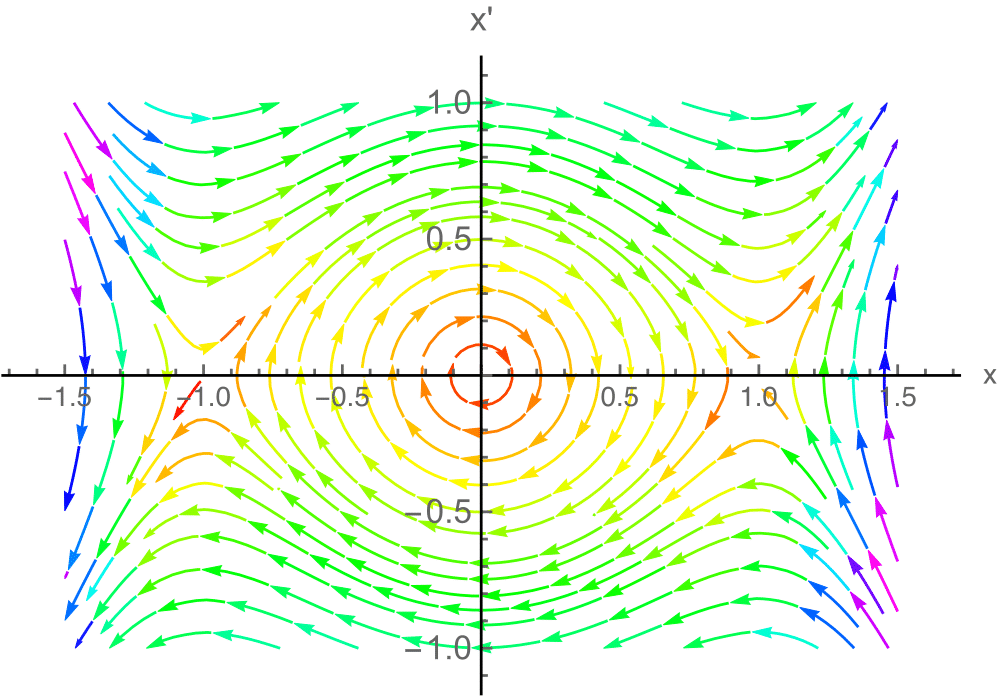
\includegraphics[scale=0.3]{figs/fig_global_stability_phase_plot_1.png}
\caption{Phase plot for $\ddot{x}+x-x^{3}=0$}
\label{fig_global_stability_phase_plot_1}
\end{figure}

Is the origin $(0,0)$ globally stable?
\begin{itemize}
\noans Yes
\noans No, it is unstable
\ans No, it is locally stable
\end{itemize}
explain

\paragraph{\textcolor{orange}{Solution:}}
This phase plot has two saddle points and a center point. The saddles are considered unstable and the circle/ellipse represents undamped oscillation, so the system is not stable.  

\paragraph{4.}
Given the dynamical system $\ddot{x}-x-x^{3}=0$, the corresponding phase plot is given by Fig.\,(\ref{fig_global_stability_phase_plot_2}).

\begin{figure}[ht]
\centering
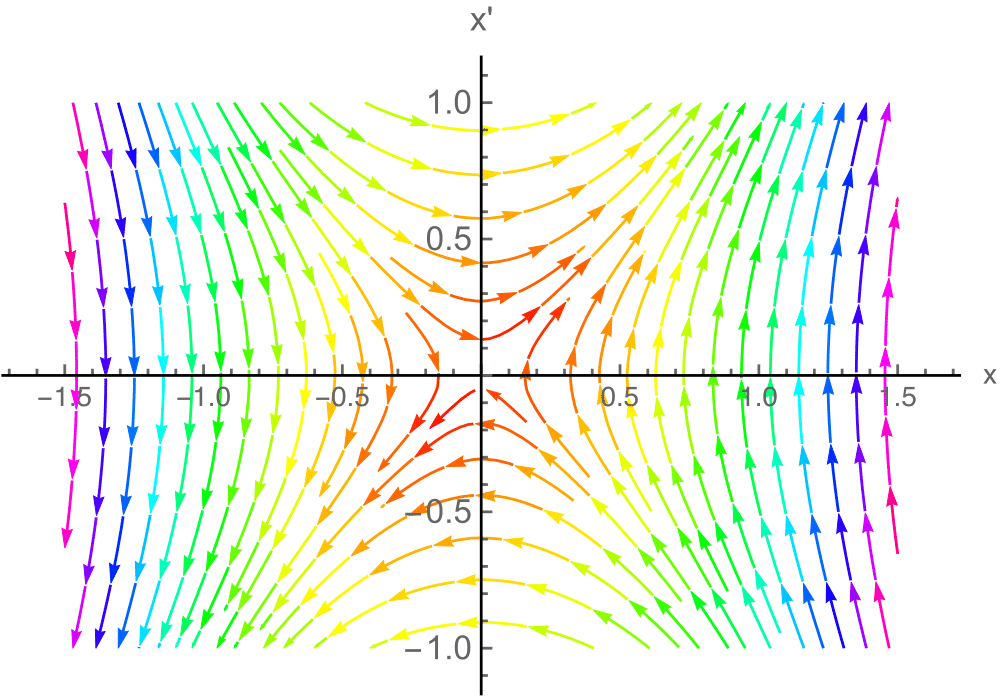
\includegraphics[scale=0.3]{figs/fig_global_stability_phase_plot_2.png}
\caption{Phase plot for $\ddot{x}-x-x^{3}=0$}
\label{fig_global_stability_phase_plot_2}
\end{figure}

Is the origin $(0,0)$ globally stable?
\begin{itemize}
\noans Yes, but only along the diagonal direction from lower left to upper right
\ans No, it is unstable
\noans It is only Lagrange stable
\end{itemize}

\paragraph{\textcolor{orange}{Solution:}}
Given phase portrait is known as saddle because of its shape. There are two converging lines and two diverging lines going to and from the saddle point respectively. This phase plot shows unstable nature of the system because the trajectory gets ejected away whenever it passes through or get near the saddle point.

\paragraph{5.}
Given the dynamical system $\ddot{x}+x+x^{3}=0$, the corresponding phase plot is given by Fig.\,(\ref{fig_global_stability_phase_plot_3}).

\begin{figure}[ht]
\centering
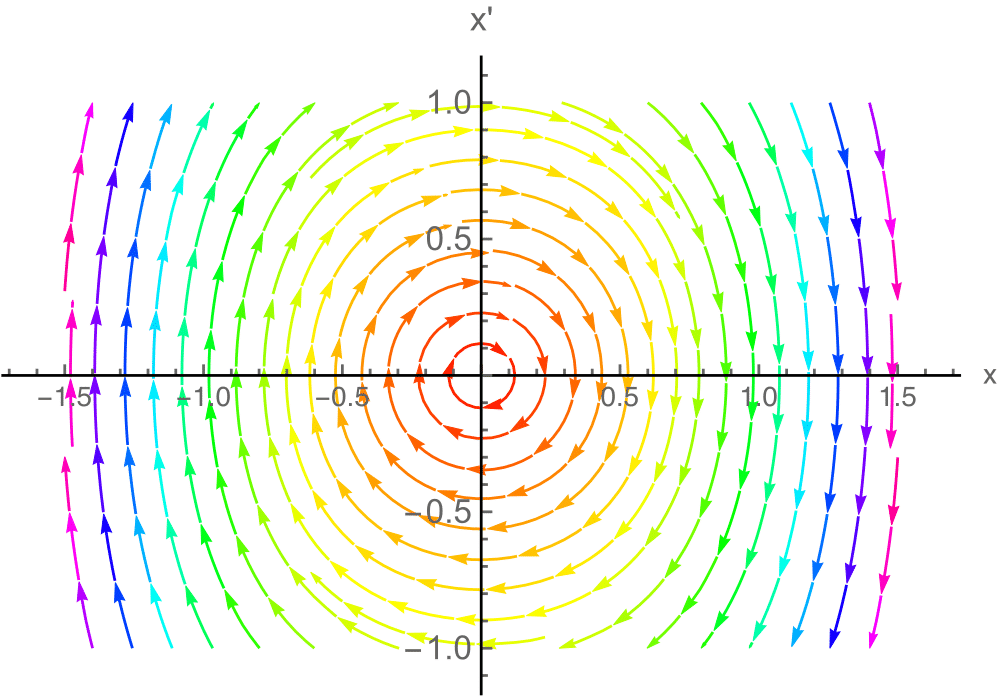
\includegraphics[scale=0.3]{figs/fig_global_stability_phase_plot_3.png}
\caption{Phase plot for $\ddot{x}+x+x^{3}=0$}
\label{fig_global_stability_phase_plot_3}
\end{figure}

Is the origin $(0,0)$ globally stable?
\begin{itemize}
\ans Yes, the motion is stable for all initial conditions
\noans No, the system contains an $x^3$ term which always leads to instability
\noans No, it is only locally stable
\end{itemize}
explain

\paragraph{\textcolor{orange}{Solution:}}
The circular/elliptical trajectory represents the perpetual oscillation around the center point. This is the nature of phase plot shown by undamped mass-spring system.

\newpage
\subsection{Linearization}
\paragraph{1.}
Linearize the MRP differential kinematic equations about a zero rotation

\begin{itemize}
\ans $\dot{\bm{\sigma}} \approx \bm{\omega}/4$
\noans $\dot{\bm{\sigma}} \approx \bm{\omega}$
\noans $\dot{\bm{\sigma}} \approx \bm{\omega}/2$
\end{itemize}

\paragraph{\textcolor{orange}{Solution:}}
Kinematic differential equation for MRP is
$$
\dot{\bm{\sigma}} = \bm{f}(\bm{\sigma},\bm{w}) = \frac{1}{4}
\begin{bmatrix}
    1-\sigma^{2}+2\sigma_{1}^{2} && 2(\sigma_{1}\sigma_{2}-\sigma_{3}) && 2(\sigma_{1}\sigma_{3}+\sigma_{2}) \\
    2(\sigma_{2}\sigma_{1}+\sigma_{3}) && 1-\sigma^{2}+2\sigma_{2}^{2} && 2(\sigma_{2}\sigma_{3}-\sigma_{1}) \\
    2(\sigma_{3}\sigma_{1}+\sigma_{2}) && 2(\sigma_{3}\sigma_{2}+\sigma_{1}) && 1-\sigma^{2}+2\sigma_{3}^{2} \\
\end{bmatrix}
\begin{bmatrix}
  \omega_{1}\\\omega_{2}\\\omega_{3}
\end{bmatrix}
$$

where $\sigma^{2}=\sigma_{1}^{2}+\sigma_{2}^{2}+\sigma_{3}^{2}$ and $\omega_{1}$, $\omega_{2}$, and $\omega_{3}$ are angular velocities.

We can write the matrix equation as the set of three differential equations:

\begin{equation*}
    \begin{split}
        \sigma_{1}&=f_{1}=\{\omega_{1}(1-\sigma^{2}+2\sigma_{1}^{2})+2\omega_{2}(\sigma_{1}\sigma_{2}-\sigma_{3})+2\omega_{3}(\sigma_{1}\sigma_{3}+\sigma_{2})\}/4 \\
        \sigma_{2}&=f_{2}=\{2\omega_{1}(\sigma_{2}\sigma_{1}+\sigma_{3})+\omega_{2}(1-\sigma^{2}+2\sigma_{2}^{2})+2\omega_{3}(\sigma_{2}\sigma_{3}-\sigma_{1})\}/4 \\
        \sigma_{3}&=f_{3}=\{2\omega_{1}(\sigma_{3}\sigma_{1}+\sigma_{2})+2\omega_{2}(\sigma_{3}\sigma_{2}+\sigma_{1})+\omega_{3}(1-\sigma^{2}+2\sigma_{3}^{2})\}/4 \\
    \end{split}
\end{equation*}

The linearized dynamics about zero rotation (i.e. $\bm{\sigma}_{r}=\bm{\omega}_{r}=\bm{0} \implies \delta\bm{\sigma}=\bm{\sigma}$ and $\delta\bm{\omega}=\bm{\omega}$) is
$$
\dot{\bm{\sigma}}\approx[\bm{A}]\bm{\sigma}+[\bm{B}]\bm{\omega}
$$

where $[\bm{A}]$ and $[\bm{B}]$ are the Jacobian matrices defined as follows.

\begin{equation}
    [\bm{A}] = 
    \begin{bmatrix}
        \frac{\partial f_{1}}{\partial\sigma_{1}} && \frac{\partial f_{1}}{\partial\sigma_{2}} && \frac{\partial f_{1}}{\partial\sigma_{3}}\\ \\
        \frac{\partial f_{2}}{\partial\sigma_{1}} && \frac{\partial f_{2}}{\partial\sigma_{2}} && \frac{\partial f_{2}}{\partial\sigma_{3}}\\ \\
        \frac{\partial f_{3}}{\partial\sigma_{1}} && \frac{\partial f_{3}}{\partial\sigma_{2}} && \frac{\partial f_{3}}{\partial\sigma_{3}}\\
    \end{bmatrix}_{\bm{\sigma}_{r},\,\bm{\omega}_{r}}
    \quad\quad
    [\bm{B}] = 
    \begin{bmatrix}
        \frac{\partial f_{1}}{\partial\omega_{1}} && \frac{\partial f_{1}}{\partial\omega_{2}} && \frac{\partial f_{1}}{\partial\omega_{3}}\\ \\
        \frac{\partial f_{2}}{\partial\omega_{1}} && \frac{\partial f_{2}}{\partial\omega_{2}} && \frac{\partial f_{2}}{\partial\omega_{3}}\\ \\
        \frac{\partial f_{3}}{\partial\omega_{1}} && \frac{\partial f_{3}}{\partial\omega_{2}} && \frac{\partial f_{3}}{\partial\omega_{3}}\\
    \end{bmatrix}_{\bm{\sigma}_{r},\,\bm{\omega}_{r}}.
\end{equation}

Let us compute $[\bm{A}]$ and $[\bm{B}]$:
$$
[\bm{A}]=\frac{1}{2}
\begin{bmatrix}
    \omega_{1}\sigma_{1}+\omega_{2}\sigma_{2}+\omega_{3}\sigma_{3}&&-\omega_{1}\sigma_{2}+\omega_{2}\sigma_{1}+\omega_{3}&&-\omega_{1}\sigma_{3}-\omega_{2}+\omega_{3}\sigma_{1}\\
    \omega_{1}\sigma_{2}-\omega_{2}\sigma_{1}+\omega_{3}&&\omega_{1}\sigma_{1}+\omega_{2}\sigma_{2}+\omega_{3}\sigma_{3}&&\omega_{1}-\omega_{2}\sigma_{3}+\omega_{3}\sigma_{2}\\
    \omega_{1}\sigma_{3}+\omega_{2}-\omega_{3}\sigma_{1}&&-\omega_{1}+\omega_{2}\sigma_{3}-\omega_{3}\sigma_{2}&&-\omega_{1}\sigma_{1}+\omega_{2}\sigma_{2}+\omega_{3}\sigma_{3}\\
\end{bmatrix}_{\bm{\sigma}_{r},\,\bm{\omega}_{r}}
= [\bm{0}]_{3\times 3}
$$
$$
[\bm{B}]=\frac{1}{4}
\begin{bmatrix}
    1-\sigma^{2}+2\sigma_{1}^{2} && 2(\sigma_{1}\sigma_{2}-\sigma_{3}) && 2(\sigma_{1}\sigma_{3}+\sigma_{2}) \\
    2(\sigma_{2}\sigma_{1}+\sigma_{3}) && 1-\sigma^{2}+2\sigma_{2}^{2} && 2(\sigma_{2}\sigma_{3}-\sigma_{1}) \\
    2(\sigma_{3}\sigma_{1}+\sigma_{2}) && 2(\sigma_{3}\sigma_{2}+\sigma_{1}) && 1-\sigma^{2}+2\sigma_{3}^{2} \\
\end{bmatrix}_{\bm{\sigma}_{r},\,\bm{\omega}_{r}}
=\frac{1}{4}[\bm{I}]_{3\times 3}
$$

Finally we get the linearized dynamics using $\dot{\bm{\sigma}}\approx[\bm{A}]\bm{\sigma}+[\bm{B}]\bm{\omega}$
$$
\dot{\bm{\sigma}}\approx\bm{\omega}/4
$$

\paragraph{2.}
Use a Taylor Series expansion to linearize $[\bm{I}]\dot{\bm{\omega}} = -[\tilde{\bm{\omega}}][\bm{I}]\bm{\omega} + \bm{L}$ about a zero rate and torque vector

\begin{itemize}
\ans $[\bm{I}]\delta\dot{\bm{\omega}} =\delta \bm{L}$
\noans $[\bm{I}]\delta\dot{\bm{\omega}} =[\bm{I}]\delta\bm{\omega} + \delta \bm{L}$
\noans $[\bm{I}]\delta\dot{\bm{\omega}} =[\bm{I}]\bm{\omega} + \delta \bm{L}$
\end{itemize}

\paragraph{\textcolor{orange}{Solution:}}
Let us suppose $\bm{f}(\bm{\omega},\bm{L})=[\bm{I}]\dot{\bm{\omega}}=-[\tilde{\bm{\omega}}][\bm{I}]\bm{\omega}+\bm{L}$. Performing Taylor series expansion of $\bm{\omega}$ about $(\bm{\omega}_{r}, \bm{L}_{r})$,
$$
[\bm{\bm{I}}]\,\delta\dot{\bm{\omega}} = \frac{\partial\bm{f}(\bm{\omega},\bm{L})}{\partial \bm{\omega}}\biggr\rvert_{\bm{\omega}_{r},\bm{L}_{r}}\delta\bm{\omega}+\frac{\partial\bm{f}(\bm{\omega},\bm{L})}{\partial\bm{L}}\biggr\rvert_{\bm{\omega}_{r},\bm{L}_{r}}\delta\bm{L} + \textnormal{ H.O.T.}
$$

Computing partial derivatives in each terms

\begin{equation*}
    \begin{split}
        \frac{\partial\bm{f}(\bm{\omega},\bm{L})}{\partial\bm{\omega}}
        &=\frac{\partial}{\partial\bm{\omega}}\left(-[\tilde{\bm{\omega}}][\bm{I}]\bm{\omega}+\bm{L}\right)\\
        &=-\frac{\partial}{\partial\bm{\omega}}(\bm{\omega}\times[\bm{I}]\bm{\omega})+\frac{\partial\bm{L}}{\partial\bm{\omega}}\\
        &=-\frac{\partial\bm{\omega}}{\partial\bm{\omega}}\times[\bm{I}]\bm{\omega}-\bm{\omega}\times\frac{\partial}{\partial\bm{\omega}}[\bm{I}]\bm{\omega}\\
        &=-[\bm{I}]\bm{\omega}-\bm{\omega}\times\left(\bm{\omega}\frac{\partial[\bm{I}]}{\partial\bm{\omega}}+\bm{[I]}\frac{\partial\bm{\omega}}{\partial\bm{\omega}}\right)\\
        &=-[\bm{I}]\bm{\omega}-\bm{\omega}\times[\bm{I}]
    \end{split}
\end{equation*}

and

\begin{equation*}
    \begin{split}
        \frac{\partial\bm{f}(\bm{\omega},\bm{L})}{\partial\bm{L}}
        &=\frac{\partial}{\partial\bm{L}}\left(-[\tilde{\bm{\omega}}][\bm{I}]\bm{\omega} + \bm{L}\right)\\
        &=1.
    \end{split}
\end{equation*}

Ignoring the H.O.T. and using these partial derivative into the Taylor expansion, we get the linearized dynamics. $(\bm{\omega}_{r}=0,\,\bm{L}_{r}=0)$

\begin{equation*}
    \begin{split}
        [\bm{I}]\,\delta\dot{\bm{\omega}}
        &=\frac{\partial\bm{f}(\bm{\omega},\bm{L})}{\partial \bm{\omega}}\biggr\rvert_{(0,0)}\delta\bm{\omega}+\frac{\partial\bm{f}(\bm{\omega},\bm{L})}{\partial\bm{L}}\biggr\rvert_{(0,0)}\delta\bm{L} \\
        &=-[\bm{I}]\bm{\omega}-\bm{\omega}\times[\bm{I}]\biggr\rvert_{(0,0)}\delta\bm{\omega} + \delta\bm{L}\\
        &= \delta\bm{L}
    \end{split}
\end{equation*}

\paragraph{3.}
Use a Taylor Series expansion to linearize $[\bm{I}]\dot{\bm{\omega}} = -[\tilde{\bm{\omega}}][\bm{I}]\bm{\omega} + \bm{L}$ about general reference vector $\bm{\omega}_{r}(t)$ with an equivalent $\bm{L}_{r}$ reference torque vector.

\begin{itemize}
\noans $[\bm{I}]\delta\dot{\bm{\omega}} = \left( [\widetilde{\bm{I}\bm{\omega}}] - [\tilde{\bm{\omega}}][\bm{I}] \right) \bm{\omega} + \delta \bm{L}$
\noans $[\bm{I}]\delta\dot{\bm{\omega}} =[\bm{I}]\delta\bm{\omega} + \delta \bm{L}$
\ans $[\bm{I}]\delta\dot{\bm{\omega}} = \left( [\widetilde{\bm{I}\bm{\omega}}_{r}] - [\tilde{\bm{\omega}}_{r}][\bm{I}] \right) \delta \bm{\omega} + \delta \bm{L}$
\end{itemize}  

\paragraph{\textcolor{orange}{Solution:}}
We can use the equations derived in above solution for this one too. The system after linearzation about general reference $(\bm{\bm{\omega}_{r}},\bm{L}_{r})$ is:

\begin{equation*}
    \begin{split}
        [\bm{I}]\,\delta\dot{\bm{\omega}}
        &=\frac{\partial\bm{f}(\bm{\omega},\bm{L})}{\partial \bm{\omega}}\biggr\rvert_{(\bm{\omega}_{r},\bm{L}_{r})}\delta\bm{\omega}+\frac{\partial\bm{f}(\bm{\omega},\bm{L})}{\partial\bm{L}}\biggr\rvert_{(\bm{\omega}_{r},\bm{L}_{r})}\delta\bm{L} \\
        &=\left(-[\bm{I}]\bm{\omega-\bm{\omega}\times[\bm{I}]}\right)\biggr\rvert_{(\bm{\omega}_{r},\bm{L}_{r})}\delta\bm{\omega} + \delta\bm{L}\\
        &= \left(-[\bm{I}]\bm{\omega}_{r}-\bm{\omega}_{r}\times[\bm{I}]\right)\delta\bm{\omega}+\delta\bm{L}
    \end{split}
\end{equation*}
check\_me

\newpage
\section{Week 2 - Overview of Lyapunov Stability Theory}
\subsection{Definite Function}
\textbf{In the following functions, is $V(\bm{x})$ positive definite, negative definite, in-definite, or semi-definite?}

\paragraph{1.}
$V(\bm{x}) = \frac{1}{2}(x_{1}^{2}+x_{2}^{2})$

\begin{itemize}
\ans Positive definite
\noans Indefinite
\noans Positive semi-definite
\end{itemize}

\paragraph{\textcolor{orange}{Solution:}}$\forall(\bm{x}\neq\bm{0})\,V(\bm{x})>0$ and $V(\bm{x})=0\iff\bm{x}=\bm{0}$. 

\paragraph{2.}
$V(\bm{x}) = \frac{1}{2}(x_{1}^{2}-x_{2}^{2})$

\begin{itemize}
\noans Positive definite along the $x_{1}$ axis but negative definite about $x_{2}$ axis
\noans Positive semi-definite
\ans Indefinite
\end{itemize}

\paragraph{\textcolor{orange}{Solution:}}$\forall(|x_{1}|>|x_{1}|) V(\bm{x})>0$ and $\forall(|x_{1}|<|x_{1}|) V(\bm{x})<0$. 

\paragraph{3.}
$V(\bm{x}) = \log(1+x_{1}^{2}+x_{2}^{2})$

\begin{itemize}
\ans Positive definite
\noans Indefinite
\noans Positive semi-definite
\end{itemize}

\paragraph{\textcolor{orange}{Solution:}}$\log(1)=0$ $\therefore$ $\forall(\bm{x}\neq\bm{0})\,V(\bm{x})>0$ and $V(\bm{x})\iff\bm{x}=\bm{0}$.

\paragraph{4.}
$V(\bm{x}) = \frac{1}{2}(x_{1}^{2}+4x_{2}^{2})$

\begin{itemize}
\ans Positive definite
\noans Indefinite
\noans Positive semi-definite
\end{itemize}

\paragraph{5.}
$V(\bm{x}) = \frac{1}{2}(x_{1}^{2}+4x_{2}^{2}) \, e^{-(x_{1}^{2}+4x_{2}^{2})}$

\begin{itemize}
\ans Globally positive definite
\noans Indefinite
\noans Positive semi-definite
\end{itemize}

\paragraph{\textcolor{orange}{Solution:}}$\forall(\bm{x}\neq\bm{0})\,V(\bm{x})>0$ and $V(\bm{x})=0\iff\bm{x}=\bm{0}$ and $|\bm{x}|\rightarrow\infty\implies V{(\bm{x})}\rightarrow\infty$. 

\vspace{2em}
\textbf{What is the definiteness of following matrices?}

\paragraph{6.}
$[\bm{K}] = 
\begin{bmatrix}
1.53947 & -0.0422688 & -0.190629 \\	
-0.0422688 & 1.4759 & 0.459006 \\
-0.190629 & 0.459006 & 1.48463 \\
\end{bmatrix}
$

\begin{itemize}
\ans Positive definite
\noans Positive semi-definite
\noans Negative definite
\noans Indefinite
\end{itemize}

\paragraph{\textcolor{orange}{Solution:}} $\lambda_{i}>0$ where $\lambda_{i}$ are the eigenvalues of $[\bm{K}]$ where $i=1,2,3$.

\paragraph{7.}
$[\bm{K}] = 
\begin{bmatrix}
-0.984331 &  -1.10006 & -0.478579 \\
-1.10006 & 1.03255 & 0.338318 \\
-0.478579 & 0.338318 & 1.45178 \\
\end{bmatrix}
$

\begin{itemize}
\noans Positive definite
\noans Positive semi-definite
\noans Negative definite
\ans Indefinite
\end{itemize}

\paragraph{\textcolor{orange}{Solution:}} None of the following are true: $\lambda_{i}>$, $\lambda_{i}<0$, $\lambda_{i}\geq0$, $\lambda_{i}\leq0$; where $\lambda_{i}$ are the eigenvalues of $[\bm{K}]$ where $i=1,2,3$.

\paragraph{8.}
$[\bm{K}] = 
\begin{bmatrix}
-2.0353 & 0.296916 & -0.365128 \\
0.296916 & -1.10369 & -0.074481 \\
-0.365128 & -0.074481 & -2.86101 \\
\end{bmatrix}
$

\begin{itemize}
\noans Positive definite
\noans Positive semi-definite
\ans Negative definite
\noans Indefinite
\end{itemize}

\paragraph{\textcolor{orange}{Solution:}} $\lambda_{i}<0$ where $\lambda_{i}$ are the eigenvalues of $[\bm{K}]$ where $i=1,2,3$.

\newpage
\subsection{Lyapunov Functions}
\paragraph{1.}
Which of these functions cannot be a proper candidate Lyapunov function?

\begin{itemize}
    \noans $V(\bm{x}) = \bm{x}^{\intercal}\bm{x}$
    \noans $V(\bm{x}) = \bm{x}^{\intercal}\bm{x} \, e^{-|\bm{x}|}$
    \ans  $V(\bm{x}) = \sin(|\bm{x}|)$
\end{itemize}

\paragraph{\textcolor{orange}{Solution:}}$\because \forall\bm{x}=[(n-1)\pi,n\pi]^{\intercal}\,\,V(\bm{x})<0\quad n=2,4,6,8...$

\paragraph{2.}
Consider the dynamical system $\ddot{x}+kx^{3}=0$. Use the Lyapunov function $V(x,\dot{x})=\frac{1}{2}\dot{x}^{2} + \frac{k}{4}x^{4}$ to study the stability about the equilibrium $x_{e} = \bm{0}$. \medskip

What is $\dot{V}$ for this case?

\begin{itemize}
    \ans $V(x,\dot{x}) = 0$
    \noans $V(x,\dot{x} = -k\dot{x}^{2})$
    \noans $V(x,\dot{x} = -kx^{2})$
\end{itemize}

\paragraph{\textcolor{orange}{Solution:}}The dynamical system and its stability analysis forms the basis for next two questions too. So I will do all the necessary derivations and arguments in this solution.

We have dynamical system $\ddot{x}+kx^{3}=0$ and Lyapunov candidate function $V(x,\dot{x})=\frac{1}{2}\dot{x}^{2} + \frac{k}{4}x^{4}$. Let us compute $\dot{V}(x,\dot{x})$.

\begin{equation*}
    \begin{split}
        \dot{V}(x,\dot{x})&=\frac{\partial V(x,\dot{x})}{\partial x}\dot{x}+\frac{\partial V(x,\dot{x})}{\partial \dot{x}}\ddot{x}\\
        &=kx^{3}\dot{x}+\dot{x}\ddot{x}\\
        &=\dot{x}(kx^{3}+\ddot{x})\\
        &=0\quad\quad\quad\quad\because\ddot{x}+kx^{3}=0\\
    \end{split}
\end{equation*}

$\dot{V}$ is always zero so is negative semi-definite (and positive semi-definite). Hence, we can conclude that the system is Lyapunov stable. 

\paragraph{3.}
Consider the dynamical system $\ddot{x}+kx^{3}=0$. Use the Lyapunov function $V(x,\dot{x})=\frac{1}{2}\dot{x}^{2} + \frac{k}{4}x^{4}$ to study the stability about the equilibrium $x_{e} = \bm{0}$. \medskip

What is definiteness of $\dot{V}$ ?

\begin{itemize}
    \noans Negative definite
    \ans Negative semi-definite
    \noans Indefinite
\end{itemize}

\paragraph{4.}
Consider the dynamical system $\ddot{x}+kx^{3}=0$. Use the Lyapunov function $V(x,\dot{x})=\frac{1}{2}\dot{x}^{2} + \frac{k}{4}x^{4}$ to study the stability about the equilibrium $\bm{x}_{e}=\bm{0}$. \medskip

What can be said about the stability of origin equilibrium point?

\begin{itemize}
    \noans It is Lagrange stable
    \ans It is Lyapunov stable
    \noans It is asymptotically stable
\end{itemize}

\paragraph{5.}
Consider the dynamical system $\ddot{x}+kx^{3}=0$. Use the Lyapunov function $V(x,\dot{x})=\frac{1}{2}\dot{x}^{2} + \frac{k}{4}x^{4}$ to study the stability about the equilibrium $\bm{x}_{e}=\bm{0}$. \medskip

What if damping is added to the dynamical system with $\ddot{x}+c\dot{x}+kx^{3}=0$ where $c$ is a positive, non-zero constant. What is $\dot{V}$ in this case?

\begin{itemize}
    \noans $\dot{V}(x,\dot{x}) = 0$
    \ans $\dot{V}(x,\dot{x}) = -c\dot{x}^{2}$
    \noans $\dot{V}(x,\dot{x}) = -cx^{2}$
\end{itemize}

\paragraph{\textcolor{orange}{Solution:}}The dynamical system and its stability analysis forms the basis for all remaining questions. So I will do all the necessary derivations and arguments in this solution.

We have dynamical system $\ddot{x}+c\dot{x}+kx^{3}=0$ and Lyapunov candidate function $V(x,\dot{x})=\frac{1}{2}\dot{x}^{2} + \frac{k}{4}x^{4}$. Let us compute $\dot{V}(x,\dot{x})$.

\begin{equation*}
    \begin{split}
        \dot{V}(x,\dot{x})&=\frac{\partial V(x,\dot{x})}{\partial x}\dot{x}+\frac{\partial V(x,\dot{x})}{\partial \dot{x}}\ddot{x}\\
        &=kx^{3}\dot{x}+\dot{x}\ddot{x}\\
        &=\dot{x}(kx^{3}+\ddot{x})\\
        &=-c\dot{x}^{2}\quad\quad\quad\quad\because\ddot{x}+kx^{3}=-c\dot{x}\\
    \end{split}
\end{equation*}

For $\dot{x}=0$, $\dot{V}(\dot{x})$ is zero for any values of $x$, otherwise it is negative. Hence $\dot{V}(\dot{x})$ is negative semi-definite. Lyapunov analysis (without considering LaSalle's theorem) suggests that the system is Lyapunov stable. Now let us compute second derivative.

\begin{equation*}
    \begin{split}
        \ddot{V}(x,\dot{x})&=\frac{\partial \dot{V}(\dot{x})}{\partial x}\dot{x}+\frac{\partial \dot{V}(\dot{x})}{\partial \dot{x}}\ddot{x}\\
        &=-2c\dot{x}\ddot{x}\\
        &=2c\dot{x}(c\dot{x}+kx^{3})\quad\quad\because\ddot{x}=-(c\dot{x}+kx^{3})\\
        &=2c^{2}\dot{x}^{2}+2kcx^{3}\dot{x}
    \end{split}
\end{equation*}

The set where $\dot{V}(\dot{x})=0$ is $\dot{x}=0$. In this set $\ddot{V}(x,\dot{x})=0$. Finally computing $\dddot{V}$.

\begin{equation*}
    \begin{split}
        \dddot{V}(x,\dot{x})&=\frac{\partial\ddot{V}(\dot{x})}{\partial x}\dot{x}+\frac{\partial \ddot{V}(\dot{x})}{\partial \dot{x}}\ddot{x}\\
        &=4c^{2}\dot{x}^{2}+2kcx^{3}\ddot{x}\\
        &=4c^{2}\dot{x}^{2}-2kcx^{3}(c\dot{x}+kx^{3})\quad\quad\because\ddot{x}=-(c\dot{x}+kx^{3})\\
        &=4c^{2}\dot{x}^{2}-2kc^{2}x^{3}\dot{x}-2ck^{2}x^{6}\\
    \end{split}
\end{equation*}

In set $\dot{x}=0$, $\ddot{V}(x,\dot{x})=-2ck^{2}x^{6}$. 

\paragraph{6.}
Consider the modified dynamical system $\ddot{x}+c\dot{x}+kx^{3}=0$. Use the Lyapunov function $V(x,\dot{x})=\frac{1}{2}\dot{x}^{2} + \frac{k}{4}x^{4}$ to study the stability about the equilibrium $\bm{x}_{e}=\bm{0}$. \medskip

With this damping, what will be the definiteness of $\dot{V}$?

\begin{itemize}
    \noans Negative definite
    \ans Negative semi-definite
    \noans Indefinite
\end{itemize}

\paragraph{7.}
Consider the modified dynamical system $\ddot{x}+c\dot{x}+kx^{3}=0$. Use the Lyapunov function $V(x,\dot{x})=\frac{1}{2}\dot{x}^{2} + \frac{k}{4}x^{4}$ to study the stability about the equilibrium $\bm{x}_{e}=\bm{0}$. \medskip

Does the damping from questions 5 and 6 prove that the system is asymptotically stable?

\begin{itemize}
    \noans Yes, damping will make anything converge
    \ans No, the proof only guarantees stability, not convergence, as $\dot{V}$ is not a function of $x$
    \noans No, $\dot{V}$ is indefinite and we can make any stability arguments
\end{itemize}

\paragraph{8.}
Consider the modified dynamical system $\ddot{x}+c\dot{x}+kx^{3}=0$. Use the Lyapunov function $V(x,\dot{x})=\frac{1}{2}\dot{x}^{2} + \frac{k}{4}x^{4}$ to study the stability about the equilibrium $\bm{x}_{e}=\bm{0}$. \medskip

To study if the system is asymptotic, what is the set where $\dot{V}$ is equal to zero?

\begin{itemize}
    \ans $\dot{x}=0$
    \noans $x=0$
    \noans Both $\dot{x}=0$ and $x=0$
\end{itemize}

\paragraph{9.}
Consider the modified dynamical system $\ddot{x}+c\dot{x}+kx^{3}=0$. Use the Lyapunov function $V(x,\dot{x})=\frac{1}{2}\dot{x}^{2} + \frac{k}{4}x^{4}$ to study the stability about the equilibrium $\bm{x}_{e}=\bm{0}$. \medskip

What is $\ddot{V}(x,\dot{x})$ for this system?

\begin{itemize}
    \noans $\ddot{V}(x,\dot{x})=-2c\dot{x}$
    \ans $\ddot{V}(x,\dot{x})=-2c\dot{x}\ddot{x}$
    \noans $\ddot{V}(x,\dot{x})=-2c\dot{x}^{2}$
\end{itemize}

\paragraph{10.}
Consider the modified dynamical system $\ddot{x}+c\dot{x}+kx^{3}=0$. Use th
e Lyapunov function $V(x,\dot{x})=\frac{1}{2}\dot{x}^{2} + \frac{k}{4}x^{4}$ to study the stability about the equilibrium $\bm{x}_{e}=\bm{0}$. \medskip

On what set where $\dot{V}$ vanished, why is $\ddot{V}$ zero here?

\begin{itemize}
    \ans Because this system is stable, $x$ and all its derivatives must be bounded. Thus, $\dot{x}$ times a bounded value will always be bounded.
    \noans Because $\dot{x} = 0$, that is enough
    \noans Because multiple terms cancel each other out, leaving zero
\end{itemize}

\paragraph{11.}
Consider the modified dynamical system $\ddot{x}+c\dot{x}+kx^{3}=0$. Use the Lyapunov function $V(x,\dot{x})=\frac{1}{2}\dot{x}^{2} + \frac{k}{4}x^{4}$ to study the stability about the equilibrium $\bm{x}_{e}=\bm{0}$. \medskip

On the set where $\dot{V}$ vanishes,what is $\ddot{V}$?

\begin{itemize}
    \noans $\ddot{V}(\dot{x}=0) = -2c^{2}kx^{2}$
    \ans $\ddot{V}(\dot{x}=0) = -2ck^{2}x^{6}$
    \noans $\ddot{V}(\dot{x}=0) = -2c^{2}\ddot{x}^{2}$
\end{itemize}

\newpage
\subsection{Asymptotic Stability}
\paragraph{1.}
For a system with $\dot{V}(x,\dot{x})=-\alpha\dot x^{2}$ with $\alpha$ being a positive constant, what is the definiteness of this function?

\begin{itemize}
    \noans It is negative definite as $-\alpha\dot{x}^{2}$ is always negative for non-zero $\dot{x}$ values
    \ans It is negative semi-definite as it is negative if $\dot{x}$ is not 0, but can be zero even if $x$ is not 0
    \noans It is indefinite as only one variable shows up
\end{itemize}

\paragraph{2.}
Consider the dynamical system $\ddot{x}+c\dot{x}+kx^{3}=0$. Use the Lyapunov function $V(x,\dot{x})=\dot{x}^{2} + \frac{k}{4}x^{4}$ to study the stability about the equilibrium $\bm{x}_{e}=\bm{0}$. \medskip

With this damping, what will be the definiteness of $\dot{V}$?

\begin{itemize}
    \noans Negative definite
    \ans Negative semi-definite
    \noans Indefinite
\end{itemize}

\paragraph{3.}
Consider the dynamical system $\ddot{x}+c\dot{x}+kx^{3}=0$. Use the Lyapunov function $V(x,\dot{x})=\dot{x}^{2} + \frac{k}{4}x^{4}$ to study the stability about the equilibrium $\bm{x}_{e}=\bm{0}$. \medskip

Does the definiteness of $\dot{V}$ prove that the system is asymptotically stable?

\begin{itemize}
    \noans Yes, damping will make anything converge
    \ans no, the proof only guarantees stability, not converge, as $\dot{V}$ is not a function of $x$
    \noans No, $\dot{V}$ is indefinite and we can't make any stability arguments
\end{itemize}

\paragraph{4.}
Consider the dynamical system $\ddot{x}+c\dot{x}+kx^{3}=0$. Use the Lyapunov function $V(x,\dot{x})=\dot{x}^{2} + \frac{k}{4}x^{4}$ to study the stability about the equilibrium $\bm{x}_{e}=\bm{0}$. \medskip

To study if the system is asymptotic, what is the set where $\dot{V}$ is equal to zero?

\begin{itemize}
    \ans $\dot{x} = 0$
    \noans $x = 0$
    \noans Both $\dot{x} = 0$ and $x = 0$
\end{itemize}

\paragraph{5.}
Consider the dynamical system $\ddot{x}+c\dot{x}+kx^{3}=0$. Use the Lyapunov function $V(x,\dot{x})= \dot{x}^{2} + \frac{k}{4}x^{4}$ to study the stability about the equilibrium $\bm{x}_{e}=\bm{0}$. \medskip

What is $\ddot{V}(x,\dot{x})$ for this system?

\begin{itemize}
    \noans $\ddot{V}(x,\dot{x})=-4c\dot{x}$
    \ans $\ddot{V}(x,\dot{x})=-4c\dot{x}\ddot{x}$
    \noans $\ddot{V}(x,\dot{x})=-4c\dot{x}^{2}$
\end{itemize}

\paragraph{6.}
Consider the dynamical system $\ddot{x}+c\dot{x}+kx^{3}=0$. Use the Lyapunov function $V(x,\dot{x})=\frac{1}{2}\dot{x}^{2} + \frac{k}{4}x^{4}$ to study the stability about the equilibrium $\bm{x}_{e}=\bm{0}$. \medskip

On what set where $\dot{V}$ vanished, why is $\ddot{V}$ zero here?

\begin{itemize}
    \ans Because this system is stable, $x$ and all its derivatives must be bounded. Thus, $\dot{x}$ times a bounded value will always be bounded.
    \noans Because $\dot{x} = 0$, that is enough
    \noans Because multiple terms cancel each other out, leaving zero
\end{itemize}

\paragraph{7.}
Consider the modified dynamical system $\ddot{x}+c\dot{x}+kx^{3}=0$. Use the Lyapunov function $V(x,\dot{x})=\dot{x}^{2} + \frac{k}{4}x^{4}$ to study the stability about the equilibrium $\bm{x}_{e}=\bm{0}$. \medskip

On what set where $\dot{V}$ vanishes,what is $\ddot{V}$?

\begin{itemize}
    \noans $\dot{V}(\dot{x}=0) = -2ckx^{2}$
    \ans $\dot{V}(\dot{x}=0) = -2ck^{2}x^{6}$
    \noans $\dot{V}(\dot{x}=0) = -2ck^{2}\ddot{x}^{2}$
\end{itemize}

\newpage
\subsection{Global Stability Applications}
\paragraph{1.}
If $V(x) = \sin^{2}(x)$ is used, can this lead to a global stability argument?

\begin{itemize}
    \noans Yes, $V(x)$ is positive around the origin
    \ans No, as $V(x)$ is not positive definite for all states $x$
    \noans Can't determine global stability without further information about the dynamical system.
\end{itemize}

\paragraph{\textcolor{orange}{Solution:}}$V(x)=0$ for $x=n\pi$ where $n=0,1,2,...$ 

\paragraph{2.}
For a planar pendulum with $\ddot{\theta}+c\dot{\theta}+\sin\theta = 0$ with $c>0$, study the resulting stability. \medskip

What is the suitable Lyapunov candidate function?

\begin{itemize}
    \noans $V(\theta,\dot{\theta}) = \frac{1}{2}\dot{\theta}^{2}$
    \ans $V(\theta,\dot{\theta}) = \frac{1}{2}\dot{\theta}^{2} - (1-\cos\theta)$
    \noans $V(\theta,\dot{\theta}) = 1-\cos\theta$
\end{itemize}

\paragraph{\textcolor{orange}{Solution:}}The dynamical system and its stability analysis forms the basis for all remaining questions. So I will do all the necessary derivations and arguments in this solution.

$V(\theta,\dot{\theta})=\frac{1}{2}\dot{\theta}^{2}-(1-\cos\theta)$ is suitable candidate function because it is positive definite function for all states (considering equilibrium $\theta=\dot{\theta}=0$). The others are not suitable as they not positive definite around some neighborhood of equilibrium since they are not function of both of the state variables. We can also observe that this particular Lyapunov function is radially unbounded because the term $\dot{\theta}^{2}\rightarrow\infty$ as $|\bm{x}|\rightarrow\infty$ where $\bm{x}=[\theta,\dot{\theta}]^{\intercal}$.
 
Taking first derivative of the Lyapunov function.
\begin{equation*}
    \begin{split}
        \dot{V}(\theta,\dot{\theta})&=\frac{\partial V(\theta,\dot{\theta})}{\partial\theta}\dot{\theta}+\frac{\partial V(\theta,\dot{\theta})}{\partial\dot{\theta}}\ddot{\theta}\\
        &=-\sin{\theta}\dot{\theta}+\dot{\theta}\ddot{\theta}\\
        &=\dot{\theta}(\sin{\theta}+\ddot{\theta})\\
        &=-c\dot{\theta}^{2}\quad\quad\because\ddot{\theta}+c\dot{\theta}+\sin\theta = 0\\
    \end{split}
\end{equation*}

Examination of first derivative clearly shows that $\dot{V}(\dot{\theta})$ is negative semi-definite because $\dot{\theta}=0$ yields $\dot{V}=0$ for any value of $\theta$. If we were to argue stability using $\dot{V}(\dot{\theta})$ \textit{only}, it would be globally stable. Now let us take the second derivative.

\begin{equation*}
    \begin{split}
        \ddot{V}(\theta,\dot{\theta})&=\frac{\partial\dot{V}(\dot{\theta})}{\partial\theta}\dot{\theta}+\frac{\partial\dot{V}(\dot{\theta})}{\partial\dot{\theta}}\ddot{\theta}\\
        &=-2c\dot{\theta}\ddot{\theta}\\
        &=-2c\dot{\theta}(c\dot{\theta}+\sin{\theta})\quad\because\ddot{\theta}+c\dot{\theta}+\sin\theta = 0\\
        &=-c^{2}\dot{\theta}^{2}-2c\dot{\theta}\sin{\theta}\\
    \end{split}
\end{equation*}

We can see that $\ddot{V}(\theta,\dot{\theta})$ is zero for the set where $\dot{V}=0$. Let us proceed with third derivative.

\begin{equation*}
    \begin{split}
        \dddot{V}(\theta,\dot{\theta})&=\frac{\partial\ddot{V}(\theta,\dot{\theta})}{\partial\theta}\dot{\theta}+\frac{\partial\ddot{V}(\theta,\dot{\theta})}{\partial\dot{\theta}}\ddot{\theta}\\
        &=-2c\dot{\theta}^{2}cos\theta-(2c^{2}\dot{\theta}+2c\sin{\theta})\ddot{\theta}\\
        &=-2c\dot{\theta}^{2}cos\theta+(2c^{2}\dot{\theta}+2c\sin{\theta})(c\dot{\theta}+\sin{\theta})\quad\because\ddot{\theta}+c\dot{\theta}+\sin\theta = 0\\
        &=-2c\dot{\theta}^{2}cos\theta+2c^{3}\dot{\theta}^{2}+4c^{2}\dot{\theta}\sin{\theta}+2c\sin^{2}{\theta}\\
    \end{split}
\end{equation*}
check\_me

From this expression we can easily see that $\dddot{V}(\dot{\theta}=0)=-2c\sin^{2}{\theta}$ which is negative semi-definite for the set where $\dot{V}=0$, hence the planar pendulum is not asymptotically stable.

\paragraph{3.}
For a planar pendulum with $\ddot{\theta}+c\dot{\theta}+\sin\theta = 0$ with $c>0$, study the resulting stability. \medskip

Is this $V$ function positive definite for all angles $\theta$ and radially unbounded?

\begin{itemize}
    \ans Yes, it is positive for all angles. While $\theta$ doesn't grow to infinity, it is monotonically increasing until 180 degrees, the worst case attitude error
    \noans No, with $\theta = 360$ degrees and $\dot{\theta} = 0$ the function is again zero
    \noans Cannot tell with the information given
\end{itemize}

\paragraph{4.}
For a planar pendulum with $\ddot{\theta}+c\dot{\theta}+\sin\theta = 0$ with $c>0$, study the resulting stability. \medskip

What is $\dot{V}$ for this system?

\begin{itemize}
    \ans $\dot{V}(\theta, \dot{\theta}) = -c\dot{\theta}^{2}$
    \noans $\dot{V}(\theta, \dot{\theta}) = -\theta^{2}$
    \noans $\dot{V}(\theta, \dot{\theta}) = -0$
\end{itemize}

\paragraph{5.}
For a planar pendulum with $\ddot{\theta}+c\dot{\theta}+\sin\theta = 0$ with $c>0$, study the resulting stability by examining just $\dot{V}$ \medskip

What can be argued about the stability considering $\dot{V}$ only?
\begin{itemize}
    \noans It is locally stable
    \ans It is globally stable
    \noans It is locally asymptotically stable
\end{itemize}

\paragraph{6.}
For a planar pendulum with $\ddot{\theta}+c\dot{\theta}+\sin\theta = 0$ with $c>0$, study the resulting stability. \medskip

What is $\dddot{V}$ evaluated on the set where $\dot{V}=0$?

\begin{itemize}
    \noans $\dddot{V}(\dot{\theta}=0) = -2c(c\dot{\theta}+\sin\theta)^{2}$
    \noans $\dddot{V}(\dot{\theta}=0) = 0$
    \ans $\dddot{V}(\dot{\theta}=0) = -2c\sin^{2}\theta$
\end{itemize}

\paragraph{7.}
For a planar pendulum with $\ddot{\theta}+c\dot{\theta}+\sin\theta = 0$ with $c>0$, study the resulting stability. \medskip

What can be said about the converge of this system considering the third time derivative of $V$?

\begin{itemize}
    \ans It is locally asymptotically stable
    \noans It is globally asymptotically stable
    \noans It is not asymptotically stable
\end{itemize}

\newpage
\subsection{General Elemental Rate}
\paragraph{1.}
Consider a general mechanical system where we want to bring the rates $\dot{\bm{q}}$ to zero. The Lyapunov function is the true kinetic energy $T$, leading to the power equation $\dot{V} = \dot{\bm{q}}^{\intercal}\bm{Q}$ where $\bm{Q}$ is a generalized force or torque set. Treat $\bm{Q}$ as your control set. Which control solution will not lead to a globally asymptotically stable response?

\begin{itemize}
    \noans $\bm{Q} = -\dot{\bm{q}}$
    \ans $\bm{Q} = -[\bm{P}]\, \dot{\bm{q}}$, \! where $[\bm{P}]=[\bm{P}]^{\intercal}$ and $[\bm{P}]$ is positive semi-definite
    \noans $\bm{Q} = -\text{sign}(\dot{\bm{q}})$, \! where $\dot{\bm{q}}^{\intercal} \, \text{sign}(\dot{\bm{q}}) = \sum_{i} \dot{q}_{i} \, \text{sign}(\dot{q}_{i})$
\end{itemize}

\paragraph{\textcolor{orange}{Solution:}}$\bm{Q}=-[\bm{P}]\,\dot{\bm{q}}\implies\dot{V}=-\dot{\bm{q}}^{\intercal}\bm{Q}[\bm{P}]\,\dot{\bm{q}}$. $\dot{\bm{q}}$ is in quadratic form so $[\bm{P}]\succeq0\implies\dot{V}\geq0$ i.e. negative semi-definite. Hence, $\dot{V}$ lead to Lyapunov stable response.

\newpage
\subsection{Rigid Body Elemental Rate Lyapunov Function}
\paragraph{1.}
Consider the controlled rotational motion of a rigid body. The goal is to drive $\bm{\omega}_{\mathcal{B}/\mathcal{N}} \rightarrow \bm{0}$. Use $V(\bm{\omega}_{\mathcal{B}/\mathcal{N}}) = \frac{1}{2}\, \bm{\omega}^{\intercal}_{\mathcal{B}/\mathcal{N}} \, \bm{\omega}_{\mathcal{B}/\mathcal{N}}$ to drive a detumble control law where the Lyapunov derivative becomes $\dot{V} = -P \bm{\omega}^{\intercal}_{\mathcal{B}/\mathcal{N}} \, \bm{\omega}_{\mathcal{B}/\mathcal{N}}$

\begin{itemize}
\ans $\bm{u} = [\tilde{\bm{\omega}}_{\mathcal{B}/\mathcal{N}}][\bm{I}]\bm{\omega}_{\mathcal{B}/\mathcal{N}} - P[\bm{I}]\bm{\omega}_{\mathcal{B}/\mathcal{N}}$
\noans $\bm{u} = - P[\bm{I}]\bm{\omega}_{\mathcal{B}/\mathcal{N}}$
\noans $\bm{u} = - P\bm{\omega}_{\mathcal{B}/\mathcal{N}}$
\end{itemize}

\paragraph{\textcolor{orange}{Solution:}}
We have,
\begin{equation*}
    \begin{split}
        \textnormal{System dynamic}&:[\bm{I}]\dot{\bm{\omega}}=-\dot{\bm{\omega}}\times([\bm{I}]\bm{\omega})+\bm{u}\\
        \textnormal{Lyapunov function}&:V(\omega)=\frac{1}{2}\bm{\omega}^{\intercal}\bm{\omega}\\
    \end{split}
\end{equation*}

Computing $\dot{V}$.

\begin{equation*}
    \begin{split}
        \dot{V}(\bm{\omega})&=\frac{1}{2}\frac{d(\bm{\omega}^{\intercal}\bm{\omega})}{d\bm{\omega}}\dot{\bm{\omega}}\\
        &=\bm{\omega}^{\intercal}\dot{\bm{\omega}}\\
        &=\bm{\omega}^{\intercal}[\bm{I}]^{-1}([\bm{I}]\dot{\bm{\omega}})\\
        &=\bm{\omega}^{\intercal}[\bm{I}]^{-1}(-\dot{\bm{\omega}}\times([\bm{I}]\bm{\omega})+\bm{u})\quad\because[\bm{I}]\dot{\bm{\omega}}=-\dot{\bm{\omega}}\times([\bm{I}]\bm{\omega})+\bm{u}\\
        &=\bm{\omega}^{\intercal}(-\dot{\bm{\omega}}\times[\bm{I}]^{-1}[\bm{I}]\bm{\omega}+[\bm{I}]^{-1}\bm{u})\\
        &=\bm{\omega}^{\intercal}(-\dot{\bm{\omega}}\times\bm{\omega}+[\bm{I}]^{-1}\bm{u})\\
        &=-\dot{\bm{\omega}}\times(\bm{\omega}^{\intercal}\bm{\omega})+\bm{\omega}^{\intercal}[\bm{I}]^{-1}\bm{u}\\
        &=\bm{\omega}^{\intercal}[\bm{I}]^{-1}\bm{u}\\
    \end{split}
\end{equation*}

check\_me $[\bm{I}]^{-1}(\dot{\bm{\omega}}\times[\bm{I}]\bm{\omega})$??

We want our $\dot{V}=-P\bm{\omega}^{\intercal}\,\bm{\omega}$, so we can solve for $\bm{u}$.

\begin{equation*}
    \begin{split}
        \dot{V}&=-P\bm{\omega}^{\intercal}\,\bm{\omega}\\
        \bm{\omega}^{\intercal}[\bm{I}]^{-1}\bm{u}&=-P\bm{\omega}^{\intercal}\,\bm{\omega}\\
        [\bm{I}]^{-1}\bm{u}&=-P\,\bm{\omega}\\
        \bm{u}&=-P\,[\bm{I}]\bm{\omega}\implies-P\,[\bm{I}]\bm{\omega}_{\mathcal{B}/\mathcal{N}}\\
    \end{split}
\end{equation*}

\paragraph{2.}
Consider the detumble control $\bm{u} = - [P]\bm{\omega}_{\mathcal{B}/\mathcal{N}}$. What can be said of the robustness of this control with respect to knowledge of the spacecraft mass properties?

\begin{itemize}
\noans Even though the mass or inertia does not appear, every control implementation must know what they are to guarantee stability
\noans It is critical to know the sign of the principle inertias
\ans This control does not use the inertia tensor, thus it is very robust to spacecraft mass distribution uncertainties
\end{itemize}

\paragraph{3.}
Consider the angular velocity vector tracking problem where the control goal is $\bm{\omega}_{\mathcal{B}/\mathcal{N}} \rightarrow \bm{\omega}_{\mathcal{R}/\mathcal{N}}$. The control solution is:
$$\bm{u}=-[\bm{P}]\delta \bm{\omega} + [\tilde{\bm{\omega}}_{\mathcal{B}/\mathcal{N}}][\bm{I}]\bm{\omega}_{\mathcal{B}/\mathcal{N}} + [\bm{I}]\left(\dot{\bm{\omega}}_{\mathcal{R}/\mathcal{N}} - [\tilde{\bm{\omega}}_{\mathcal{B}/\mathcal{N}}] \bm{\omega}_{\mathcal{R}/\mathcal{N}}\right)$$.

Use the Lyapunov function
$$ V(\delta \bm{\omega}) = \frac{1}{2}\, \delta \bm{\omega}^{\intercal}[\bm{I}]\delta\bm{\omega}$$

where, $\delta\bm{\omega}=\bm{\omega}_{\mathcal{B}/\mathcal{N}}-\bm{\omega}_{\mathcal{R}/\mathcal{N}}$.

Derive the simplest corresponding Lyapunov
derivative expression:

\begin{itemize}
\ans $\dot{V} = -\delta \bm{\omega}^{\intercal}[\bm{P}]\delta\bm{\omega}$
\noans $\dot{V} = -\delta \bm{\omega}^{\intercal} \left(- [\tilde{\bm{\omega}}_{\mathcal{B}/\mathcal{N}}][\bm{I}] \bm{\omega}_{\mathcal{B}/\mathcal{N}} + [\tilde{\bm{\omega}}_{\mathcal{R}/\mathcal{N}}][\bm{I}] \bm{\omega}_{\mathcal{B}/\mathcal{N}} - [\bm{P}]\delta\bm{\omega} \right)$
\noans $\dot{V} = -\delta \bm{\omega}^{\intercal}[\bm{I}][\bm{P}]\delta{\bm{\omega}}$
\end{itemize}

\paragraph{\textcolor{orange}{Solution:}} Using shorthand notations: $\bm{\omega}_{\mathcal{B}/\mathcal{N}}=\bm{\omega}$ and $\bm{\omega}_{\mathcal{R}/\mathcal{N}}=\bm{\omega}_{r}$.
\begin{equation*}
    \begin{split}
        \dot{V}&=\frac{1}{2}\frac{\partial(\delta\bm{\omega}^{\intercal}[\bm{I}]\delta\bm{\omega})}{\partial\,\delta\bm{\omega}}\delta\dot{\bm{\omega}}\\
        &=\delta\bm{\omega}^{\intercal}\,[\bm{I}]\,\delta\dot{\bm{\omega}}\quad\quad\\
        &=\delta\bm{\omega}^{\intercal}\,[\bm{I}]\,(\dot{\bm{\omega}}-\dot{\bm{\omega}}_{r}+\bm{\omega}\times\bm{\omega}_{r})\quad\because\delta\dot{\bm{\omega}}=\frac{{}^{\mathcal{B}}d\bm{\omega}}{dt}=\dot{\bm{\omega}}-\dot{\bm{\omega}}_{r}+\bm{\omega}\times\bm{\omega}_{r}\\
        &=\delta\bm{\omega}^{\intercal}([\bm{I}]\dot{\bm{\omega}}-[\bm{I}]\dot{\bm{\omega}}_{r}+[\bm{I}]\bm{\omega}\times\bm{\omega}_{r})\\
        &=\delta\bm{\omega}^{\intercal}(-[\tilde{\bm{\omega}}][\bm{I}]\bm{\omega}-[\bm{I}]\dot{\bm{\omega}}_{r}+[\bm{I}]\bm{\omega}\times\bm{\omega}_{r}+\bm{u})\\
    \end{split}
\end{equation*}

Plugging in $\bm{u}=-[\bm{P}]\delta\bm{\omega}+[\tilde{\bm{\omega}}][\bm{I}]\bm{\omega}+[\bm{I}]\dot{\bm{\omega}}_{r}-[\bm{I}][\tilde{\bm{\omega}}]\bm{\omega}_{r}$ we get

\begin{equation*}
    \begin{split}
        \dot{V}&=\delta\bm{\omega}^{\intercal}(-[\tilde{\bm{\omega}}][\bm{I}]\bm{\omega}-[\bm{I}]\dot{\bm{\omega}}_{r}+[\bm{I}]\bm{\omega}\times\bm{\omega}_{r}-[\bm{P}]\delta\bm{\omega}+[\tilde{\bm{\omega}}][\bm{I}]\bm{\omega}+[\bm{I}]\dot{\bm{\omega}}_{r}-[\bm{I}][\tilde{\bm{\omega}}]\bm{\omega}_{r})\\
        &=\delta\bm{\omega}^{\intercal}([\bm{I}]\bm{\omega}\times\bm{\omega}_{r}-[\bm{P}]\delta\bm{\omega}-[\bm{I}][\tilde{\bm{\omega}}]\bm{\omega}_{r})\\
        &=\delta\bm{\omega}^{\intercal}([\bm{I}]\bm{\omega}\times\bm{\omega}_{r}-[\bm{P}]\delta\bm{\omega}-[\bm{I}]\bm{\omega}\times\bm{\omega}_{r})\\
        &=-\delta\bm{\omega}^{\intercal}[\bm{P}]\delta\bm{\omega}.\\
    \end{split}
\end{equation*}

\paragraph{4.}
What can be said about the stability properties of this control?
\begin{itemize}
\noans It is Lyapunov stable as $\dot{V}$ is negative semidefinite
\noans It is Lagrange stable
\ans It is asymptotically stable as $\dot{V}$ is negative definite 
\end{itemize}

\paragraph{\textcolor{orange}{Solution:}} $V(\delta\bm{\omega})\succ0$ for all $\delta\bm{\bm{\omega}}$ and we can see that $\dot{V}(\delta{\bm{\omega}})\prec0$ so this control is asymptotically stable.

\newpage
\subsection{General Elemental State Lyapunov Function}
\paragraph{1.}
Given the Lyapunov function $V(\bm{\sigma})=2K\,\text{ln}(1+\sigma^{2})$ where $\sigma^{2}=\bm{\sigma}^{\intercal}\bm{\sigma}$. What is the time derivative of this scalar function?

\begin{itemize}
\noans $\dot{V}(\bm{\sigma}) = \cfrac{4K}{1+\sigma^{2}}$
\noans $\dot{V}(\bm{\sigma}) = \cfrac{4K\bm{\sigma}}{1+\sigma^{2}}$
\ans $\dot{V}(\bm{\sigma}) = \cfrac{4K \bm{\sigma}^{\intercal}\dot{\bm{\sigma}}}{1+\sigma^{2}}$
\end{itemize}

\paragraph{\textcolor{orange}{Solution:}}
\begin{equation*}
    \begin{split}
        \dot{\bm{V}}(\bm{\sigma})&=\frac{\partial V}{\partial\bm{\sigma}}\dot{\bm{\sigma}}\\
        &=\frac{\partial\,(2K\,\text{ln}(1+\sigma^{2}))}{\partial\bm{\sigma}}\dot{\bm{\sigma}}\\
        &=2K\frac{\partial\,(\text{ln}(1+\sigma^{2}))}{\partial(1+\sigma^{2})}\frac{\partial(1+\sigma^{2})}{\partial\bm{\sigma}}\dot{\bm{\sigma}}\\
        &=\frac{2K}{1+\sigma^{2}}\frac{\partial(1+\bm{\sigma}^{\intercal}\bm{\sigma})}{\partial\bm{\sigma}}\dot{\bm{\sigma}}\\
        &=\frac{4K}{1+\sigma^{2}}\bm{\sigma}^{\intercal}\dot{\bm{\sigma}}
    \end{split}
\end{equation*}

\paragraph{2.} Substitute in the MRP differential kinematic equation for $\dot{\bm{\sigma}}$ and simplify.

\begin{itemize}
\noans $\dot{V}(\bm{\sigma}) = K\cfrac{\bm{\sigma}^{\intercal}\left((1-\sigma^{2})[\bm{I}_{3\times3}]+2[\tilde{\bm{\sigma}}]+2\bm{\sigma}\bm{\sigma}^{\intercal}\right)\bm{\omega}}{1+\sigma^{2}}$
\ans $\dot{V}(\bm{\sigma}) = K\bm{\sigma}^{\intercal}\bm{\omega}$
\noans $\dot{V}(\bm{\sigma}) = K\bm{\sigma}^{\intercal}\bm{\omega} - \cfrac{2K}{1+\sigma^{2}}\,\bm{\sigma}^{\intercal}[\tilde{\bm{\sigma}}]\bm{\omega}$
\end{itemize}

\paragraph{\textcolor{orange}{Solution:}}
\begin{equation*}
    \begin{split}
        \dot{V}(\bm{\sigma})&=\frac{4K}{1+\sigma^{2}}\bm{\sigma}^{\intercal}\dot{\bm{\sigma}}\\
        &=\frac{4K}{1+\sigma^{2}}\bm{\sigma}^{\intercal}\frac{1}{4}\left((1-\sigma^{2})[\bm{I}_{3\times3}]+2[\tilde{\bm{\sigma}}]+2\bm{\sigma}\bm{\sigma}^{\intercal}\right)\bm{\omega}\\
        &=\frac{K}{1+\sigma^{2}}\left((1-\sigma^{2})\bm{\sigma}^{\intercal}[\bm{I}_{3\times3}]+2\bm{\sigma}^{\intercal}[\tilde{\bm{\sigma}}]+2\bm{\sigma}^{\intercal}\bm{\sigma}\bm{\sigma}^{\intercal}\right)\bm{\omega}\\
        &=\frac{K}{1+\sigma^{2}}\left((1-\sigma^{2})\bm{\sigma}^{\intercal}-2[\tilde{\bm{\sigma}}]\bm{\sigma}+2\sigma^{2}\bm{\sigma}^{\intercal}\right)\bm{\omega}\quad\because[\tilde{\bm{\sigma}}]^{\intercal}=-[\tilde{\bm{\sigma}}]\\
        &=\frac{K}{1+\sigma^{2}}\left(\bm{\sigma}^{\intercal}-\sigma^{2}\bm{\sigma}^{\intercal}-2\bm{\sigma}\times\bm{\sigma}+2\sigma^{2}\bm{\sigma}^{\intercal}\right)\bm{\omega}\\
        &=\frac{K}{1+\sigma^{2}}\left(\bm{\sigma}^{\intercal}+\sigma^{2}\bm{\sigma}^{\intercal}\right)\bm{\omega}\\
        &=\frac{K}{1+\sigma^{2}}\bm{\sigma}^{\intercal}\left(1+\sigma^{2}\right)\bm{\omega}\\
        &=K\bm{\sigma}^{\intercal}\bm{\omega}\\
    \end{split}
\end{equation*}

\newpage
\section{Week 3 - Attitude Control of States and Rates}
\subsection{General 3-Axis Attitude Control}
\paragraph{1.}
Consider the general 3-axis control where the goal is to drive $\bm{\sigma}_{\mathcal{B}/\mathcal{N}} \rightarrow 0$ and  $\bm{\omega}_{\mathcal{B}/\mathcal{N}} \rightarrow 0$. Use the Lyapunov function:
$$V(\bm{\sigma}_{\mathcal{B}/\mathcal{N}},\bm{\omega}_{\mathcal{B}/\mathcal{N}}) = \frac{1}{2}\,\bm{\omega}^{\intercal}_{\mathcal{B}/\mathcal{N}}[\bm{I}]\bm{\omega}_{\mathcal{B}/\mathcal{N}} + 2K\, \text{ln} \left( 1 + \bm{\sigma}^{\intercal}_{\mathcal{B}/\mathcal{N}}\bm{\sigma}_{\mathcal{B}/\mathcal{N}} \right)$$

What is the Lyapunov rate if the control is 
$$\bm{u} = -K \bm{\sigma}_{\mathcal{B}/\mathcal{N}} - [\bm{P}]\bm{\omega}_{\mathcal{B}/\mathcal{N}}?$$

\begin{itemize}
\ans $\dot{V}(\bm{\sigma}_{\mathcal{B}/\mathcal{N}},\bm{\omega}_{\mathcal{B}/\mathcal{N}}) = -\bm{\omega}^{\intercal}_{\mathcal{B}/\mathcal{N}}[\bm{P}]\bm{\omega}_{\mathcal{B}/\mathcal{N}}$
\noans $\dot{V}(\bm{\sigma}_{\mathcal{B}/\mathcal{N}},\bm{\omega}_{\mathcal{B}/\mathcal{N}}) = -\bm{\omega}^{\intercal}_{\mathcal{B}/\mathcal{N}}\bm{\omega}_{\mathcal{B}/\mathcal{N}}$
\noans $\dot{V}(\bm{\sigma}_{\mathcal{B}/\mathcal{N}},\bm{\omega}_{\mathcal{B}/\mathcal{N}}) = -\bm{\omega}^{\intercal}_{\mathcal{B}/\mathcal{N}}\bm{\omega}_{\mathcal{B}/\mathcal{N}} - \bm{\sigma}^{\intercal}_{\mathcal{B}/\mathcal{N}}\bm{\sigma}_{\mathcal{B}/\mathcal{N}}$
\end{itemize}

\paragraph{\textcolor{orange}{Solution:}}
\begin{equation*}
    \begin{split}
        \dot{V}(\bm{\sigma}_{\mathcal{B}/\mathcal{N}},\bm{\omega}_{\mathcal{B}/\mathcal{N}}) &= \frac{\partial V}{\partial\bm{\sigma}}\dot{\bm{\sigma}} + \frac{\partial V}{\partial\bm{\omega}}\dot{\bm{\omega}}\\
        &= K\bm{\omega}^{\intercal}\bm{\sigma} + \bm{\omega}^{\intercal}[\bm{I}]\dot{\bm{\omega}}\\
        &= K\bm{\omega}^{\intercal}\bm{\sigma} + \bm{\omega}^{\intercal}(-\bm{\omega}\times[\bm{I}]\bm{\omega} + \bm{u})\\
        &= K\bm{\omega}^{\intercal}\bm{\sigma} + \bm{\omega}^{\intercal}(-\bm{\omega}\times[\bm{I}]\bm{\omega} - K\bm{\sigma}-[\bm{P}]\bm{\omega})\\
        &= K\bm{\omega}^{\intercal}\bm{\sigma} + \bm{\omega}^{\intercal}(-[\tilde{\bm{\omega}}][\bm{I}]\bm{\omega} - K\bm{\sigma}-[\bm{P}]\bm{\omega})\\
        &= K\bm{\omega}^{\intercal}\bm{\sigma} - \bm{\omega}^{\intercal}[\tilde{\bm{\omega}}][\bm{I}]\bm{\omega} - K\bm{\omega}^{\intercal}\bm{\sigma}-\bm{\omega}^{\intercal}[\bm{P}]\bm{\omega}\quad\because \bm{\omega}^{\intercal}[\tilde{\bm{\omega}}]=0\\
        &=-\bm{\omega}^{\intercal}[\bm{P}]\bm{\omega}\\
    \end{split}
\end{equation*}

\paragraph{2.}
What is the Lyapunov rate if the control is
$$\bm{u} = -K \bm{\sigma}_{\mathcal{B}/\mathcal{N}} - [\bm{P}]\bm{\omega}_{\mathcal{B}/\mathcal{N}} + [\tilde{\bm{\omega}}_{\mathcal{B}/\mathcal{N}}][\bm{I}]\bm{\omega}_{\mathcal{B}/\mathcal{N}}?$$

\begin{itemize}
\ans $\dot{V}(\bm{\sigma}_{\mathcal{B}/\mathcal{N}},\bm{\omega}_{\mathcal{B}/\mathcal{N}}) = -\bm{\omega}^{\intercal}_{\mathcal{B}/\mathcal{N}}[\bm{P}]\bm{\omega}_{\mathcal{B}/\mathcal{N}}$
\noans $\dot{V}(\bm{\sigma}_{\mathcal{B}/\mathcal{N}},\bm{\omega}_{\mathcal{B}/\mathcal{N}}) = -\bm{\omega}^{\intercal}_{\mathcal{B}/\mathcal{N}}\bm{\omega}_{\mathcal{B}/\mathcal{N}}$
\noans $\dot{V}(\bm{\sigma}_{\mathcal{B}/\mathcal{N}},\bm{\omega}_{\mathcal{B}/\mathcal{N}}) = -\bm{\omega}^{\intercal}_{\mathcal{B}/\mathcal{N}}\bm{\omega}_{\mathcal{B}/\mathcal{N}} - \bm{\sigma}^{\intercal}_{\mathcal{B}/\mathcal{N}}\bm{\sigma}_{\mathcal{B}/\mathcal{N}}$
\end{itemize}

\paragraph{\textcolor{orange}{Solution:}}
\begin{equation*}
    \begin{split}
        \dot{V}(\bm{\sigma}_{\mathcal{B}/\mathcal{N}},\bm{\omega}_{\mathcal{B}/\mathcal{N}}) &= \frac{\partial V}{\partial\bm{\sigma}}\dot{\bm{\sigma}} + \frac{\partial V}{\partial\bm{\omega}}\dot{\bm{\omega}}\\
        &= K\bm{\omega}^{\intercal}\bm{\sigma} + \bm{\omega}^{\intercal}[\bm{I}]\dot{\bm{\omega}}\\
        &= K\bm{\omega}^{\intercal}\bm{\sigma} + \bm{\omega}^{\intercal}(-\bm{\omega}\times[\bm{I}]\bm{\omega} + \bm{u})\\
        &= K\bm{\omega}^{\intercal}\bm{\sigma} + \bm{\omega}^{\intercal}(-\bm{\omega}\times[\bm{I}]\bm{\omega} - K\bm{\sigma}-[\bm{P}]\bm{\omega} + [\tilde{\bm{\omega}}][\bm{I}]\bm{\omega})\\
        &= K\bm{\omega}^{\intercal}\bm{\sigma} + \bm{\omega}^{\intercal}(-[\tilde{\bm{\omega}}][\bm{I}]\bm{\omega} - K\bm{\sigma}-[\bm{P}]\bm{\omega} + [\tilde{\bm{\omega}}][\bm{I}]\bm{\omega})\\
        &= K\bm{\omega}^{\intercal}\bm{\sigma} - K\bm{\omega}^{\intercal}\bm{\sigma}-\bm{\omega}^{\intercal}[\bm{P}]\bm{\omega}\\
        &=-\bm{\omega}^{\intercal}[\bm{P}]\bm{\omega}\\
    \end{split}
\end{equation*}

\paragraph{3.}
What is the difference between these two attitude control solutions?

\begin{itemize}
\noans The first one is more strongly stable
\noans The second on is more stable, but has less performance
\ans The closed loop performance is the only difference.  Both have the same stability guarantees
\end{itemize}

\paragraph{4.}
Write software code to simulate the general spacecraft motion where a control torque $\bf{u}$ is being applied. The principal inertias are $I_{1} = 100$ kgm$^{2}$, $I_{2} = 75$ kgm$^{2}$ and $I_{3} = 80$ kgm$^{2}$. The initial states are
$$\bm{\sigma}_{\mathcal{B}/\mathcal{N}}(t_{o}) = (0.1,0.2,-0.1)\text{ and }\bm{\omega}_{\mathcal{B}/\mathcal{N}}(t_{o}) = (30,10,-20) \text{ deg/sec.}$$

Use the globally asymptotically stabilizing control solution:
$$\bm{u} = -K\bm{\sigma}_{\mathcal{B}/\mathcal{R}} - [\bm{P}]\bm{\omega}_{\mathcal{B}/\mathcal{R}} + [\bm{I}]\left(\dot{\bm{\omega}}_{\mathcal{R}/\mathcal{N}} - \bm{\omega}_{\mathcal{B}/\mathcal{N}}\times\bm{\omega}_{\mathcal{R}/\mathcal{N}}\right) + [\tilde{\bm{\omega}}_{\mathcal{B}/\mathcal{N}}][\bm{I}]\bm{\omega}_{\mathcal{B}/\mathcal{N}} - \bm{L}$$

Use the gains $K = 5$ Nm and $P = 10$ Nms where $[\bm{P}] = P [\bm{I}_{3\times3}]$. For the following case, assume $\bm{L}$ is zero. \medskip

Simulate a regulator case (i.e. reference frame is equal to inertial frame) for the 120 seconds where $\bm{\sigma}_{\mathcal{B}/\mathcal{N}}$ is the zero orientation. Enter below the MRP norm $\sqrt{\sigma_{1}^{2}+\sigma_{2}^{2}+\sigma_{3}^{2}}$ at 30 seconds into the simulation.

\paragraph{\textcolor{orange}{Solution:}}0.195263

\paragraph{5.}
Simulate an attitude tracking care for 120 seconds where
\begin{center}
$\bm{\sigma}_{\mathcal{R}/\mathcal{N}} = \left(0.2\sin(ft),0.3\cos(ft),-0.3\sin(ft)\right)$ with $f=0.05$ rad/sec.
\end{center}
Enter below the MRP tracking error norm $|\bm{\sigma}_{\mathcal{B}/\mathcal{N}}|$ at 40 seconds into the simulation.

\paragraph{\textcolor{orange}{Solution:}}0.159240

\newpage
\subsection{Asymptotic Stability}
\paragraph{1.}
In the shown control development, why is $\dot{V}(\bm{\sigma},\delta\bm{\omega}) = -\delta\bm{\omega}^{\intercal}[\bm{P}] \delta\bm{\omega}$ only globally negative semi-definite?

\begin{itemize}
\noans This is a trick question, it is negative definite
\ans It is negative semi-definite because $V$ is a function of both $\bm{\sigma}$ $\bm{\omega}$, but $\dot{V}$ is only negative definite in terms of $\delta\bm{\omega}$
\noans It is only negative semi-definite because the gain matrix $[\bm{P}]$ is only positive semi-definite
\end{itemize}

\paragraph{2.}
To use the Mukherjee-Chen theorem, we evaluate higher order time derivatives of $\dot{V}$ and evaluate the results on what set of sets?

\begin{itemize}
\noans Always when the rates are zero
\noans To show global stability we express the function in terms of any states
\ans On the set of states that causes $\dot{V}$ to be zero
\end{itemize}

\paragraph{3.}
For the system to be asymptotically stabilizing, which derivative must be the first non-zero derivative?

\begin{itemize}
\ans This must be an odd number
\noans This must be an even number
\noans This is always the 3$^{\text{rd}}$ derivative
\end{itemize}

\paragraph{4.}
With the Mukherjee-Chen theorem, what must be true of the first non-zero evaluated Lyapunov function derivative for the system to be asymptotically stabilizing?

\begin{itemize}
\ans This derivative expression must be negative definite in terms of the unknown states
\noans This derivative must simply be non-zero
\noans This derivative expression must be positive definite in terms of the unknown states
\end{itemize}

\paragraph{5.}
Write software code to simulate the general spacecraft motion where a control torque $\bf{u}$ is being applied. The principal inertias are $I_{1} = 100$ kgm$^{2}$, $\bm{I}_{2} = 75$ kgm$^{2}$ and $I_{3} = 80$ kgm$^{2}$. The initial states are
$$\bm{\sigma}_{\mathcal{B}/\mathcal{N}}(t_{o}) = (0.1,0.2,-0.1)\text{ and }\bm{\omega}_{\mathcal{B}/\mathcal{N}}(t_{o}) = (30,10,-20) \text{ deg/sec.}$$

Use the gains $K = 5$ Nm and $P = 10$ Nms where $[\bm{P}] = P [\bm{I}_{3\times3}]$. The reference attitude is given by
$$\bm{\sigma}_{\mathcal{R}/\mathcal{N}} = \left(0.2\,\sin(ft),0.3\,\cos(ft),-0.3\sin(ft)\right)\text{ with }f = 0.05 \text{ rad/sec.}$$

Simulate the attitude response if the control is simply
$$\bm{u} = -K\bm{\sigma}_{\mathcal{B}/\mathcal{R}}-[\bm{P}]\bm{\omega}_{\mathcal{B}/\mathcal{R}}.$$

Assume no external  torque is present. What is the tracking error MRP norm $|\bm{\sigma}_{B/R}|$ at 20 seconds into the simulation?

\paragraph{\textcolor{orange}{Solution:}}0.378330

\paragraph{6.}
Simulate the attitude response if the control is
$$\bm{u} = -K\bm{\sigma}_{\mathcal{B}/\mathcal{R}} - [\bm{P}]\bm{\omega}_{\mathcal{B}/\mathcal{R}} + [\bm{I}](\dot{\bm{\omega}}_{\mathcal{R}/\mathcal{N}} - \bm{\omega}_{\mathcal{B}/\mathcal{N}} \times \bm{\omega}_{\mathcal{R}/\mathcal{N}}) + [\tilde{\bm{\omega}}_{\mathcal{B}/\mathcal{N}}][\bm{I}]\bm{\omega}_{\mathcal{B}/\mathcal{N}} - \bm{L}$$

Model an external torque of $\bm{L}=(0.5,-0.3,0.2)$ Nm. What is the tracking error MRP norm $|\bm{\sigma}_{B/R}|$ at 80 seconds into the simulation?

\paragraph{\textcolor{orange}{Solution:}}0.134425

\paragraph{7.}
Simulate the attitude response if the control is
$$\bm{u} = -K\bm{\sigma}_{\mathcal{B}/\mathcal{R}} - [\bm{P}]\bm{\omega}_{\mathcal{B}/\mathcal{R}} + [\bm{I}](\dot{\bm{\omega}}_{\mathcal{R}/\mathcal{N}} - \bm{\omega}_{\mathcal{B}/\mathcal{N}} \times \bm{\omega}_{\mathcal{R}/\mathcal{N}}) + [\tilde{\bm{\omega}}_{\mathcal{B}/\mathcal{N}}][\bm{I}]\bm{\omega}_{\mathcal{B}/\mathcal{N}} - \bm{L}$$

Assume no external torque is present. What is the tracking error MRP norm $|\bm{\sigma}_{B/R}|$ at 70 seconds into the simulation?

\paragraph{\textcolor{orange}{Solution:}}0.032280

\newpage
\subsection{Unknown External Torques}
\paragraph{1.}
With the 3-axes attitude control torque
$$\bm{u} = -K\bm{\sigma}_{\mathcal{B}/\mathcal{R}} - [\bm{P}]\bm{\omega}_{\mathcal{B}/\mathcal{R}} + [\bm{I}](\dot{\bm{\omega}}_{\mathcal{R}/\mathcal{N}} - \bm{\omega}_{\mathcal{B}/\mathcal{N}} \times \bm{\omega}_{\mathcal{R}/\mathcal{N}}) + [\tilde{\bm{\omega}}_{\mathcal{B}/\mathcal{N}}][\bm{I}]\bm{\omega}_{\mathcal{B}/\mathcal{N}} - \bm{L},$$
is it possible for unmodeled torques to drive the spacecraft towards an infinitely fast spin?

\begin{itemize}
\noans Yes, the disturbance will cause the rate errors to grow unbounded
\ans No, the $\dot{V}$ expression illustrates that the $\delta \bm{\omega}$ values must remain bounded
\noans Yes, this control is not robust without integral feedback
\end{itemize}

\paragraph{\textcolor{orange}{Solution:}} Without consideration of the unmodeled torque $\Delta L$, is designed to create $\dot{V}$ to be negative semi-definite.

$$
\dot{V} = - \delta\bm{\omega}^{\intercal}[\bm{P}]\delta\bm{\omega}
$$

However, in the presence of unmodeled torque, a new term in introduced to $\dot{V}$. 
$$
\dot{V} = - \delta\dot{\bm{\omega}}[\bm{P}]\delta\bm{\omega} + \delta\bm{\omega}^{\intercal}\Delta \bm{L}
$$

Introduction of  $\delta\bm{\omega}^{\intercal}\Delta\bm{L}$ changes the $\dot{V}$ to indefinite function. This clearly suggests that the control does not guarantee stability for $\delta\bm{\omega}$. However, observation of $\dot{V}$ suggests that $\Delta\bm{L}$ cannot drive to rates to infinity either. This is because, for large angular rates (i.e. large $\delta\bm{\omega}$), the quadratic term will dominate. When $\delta\bm{\omega}$ get large enough, at some point $\dot{V}$ will be negative and start stabilizing $\bm{\omega}$. Hence stabilizing effect will be stronger for large rates than potential destabilization due to  unmodeled torque and rates does not tend to infinity. Not only it does not blow up, actually $\delta\bm{\omega}\rightarrow0$.

\paragraph{2.}
Write software code to simulate the general spacecraft motion where a control torque $\bf{u}$ is being applied. The principal inertias are $I_{1} = 100$ kgm$^{2}$, $\bm{I}_{2} = 75$ kgm$^{2}$ and $I_{3} = 80$ kgm$^{2}$. The initial states are
$$\bm{\sigma}_{\mathcal{B}/\mathcal{N}}(t_{o}) = (0.1,0.2,-0.1)\text{ and }\bm{\omega}_{\mathcal{B}/\mathcal{N}}(t_{o}) = (30,10,-20) \text{ deg/sec.}$$

Use the gains $K = 5$ Nm and $P = 10$ Nms where $[\bm{P}] = P [\bm{I}_{3\times3}]$. The reference attitude is given by the zero orientation.

If the unknown external torque $\Delta \bm{L} = (0.5,-0.3,0.2)$Nm, what are the predicted steady state attitude errors?

\begin{itemize}
\noans $\bm{\sigma}_{ss} = (-0.1,0.06,-0.04)$
\ans $\bm{\sigma}_{ss} = (0.1,-0.06,0.04)$
\noans $\bm{\sigma}_{ss} = (-0.2,-0.12,-0.8)$
\end{itemize}

\paragraph{\textcolor{orange}{Solution:}}
$$
\bm{\sigma}_{ss} = \frac{1}{K}\Delta \bm{L} = (0.1, -0.06, 0.04)
$$

\paragraph{3.}
As there is a steady-state pointing error, this closed-loop response is ... .

\begin{itemize}
\ans Lagrange stable
\noans Lyapunov stable
\noans Globally stable
\end{itemize}

\paragraph{\textcolor{orange}{Solution:}} In the presence of constant unmodeled torque   $\Delta\bm{L}$, attitude does not converge to desired attitude but to some other attitude near it resulting steady state attitude error $\bm{\sigma}_{ss}$. In this case, our attitude never converges to the intended equilibrium attitude but remains bounded around it for all initial conditions. We have no control over values of $\bm{\sigma}_{ss}$ by choosing different initial conditions, hence the closed loop 

\paragraph{4.}
Simulate the control response and validate that the spacecraft attitude settles to this predicted steady state pointing error. What is the tracking error MRP norm $|\bm{\sigma}_{\mathcal{B}/\mathcal{R}}|$ at 35 seconds into the simulation?

\paragraph{\textcolor{orange}{Solution:}}
0.277102

\newpage
\subsection{Integral Feedback}
\paragraph{1.}
In the presented nonlinear attitude control with integral feedback, does adding the integral term impact the asymptotic convergence of the unperturbed system?

\begin{itemize}
\noans Yes, but the pointing error is typically small
\ans No, the control retains global asymptotic stability properties
\noans No, as long as the gain $K$ is made large enough  
\end{itemize}

\paragraph{\textcolor{orange}{Solution:}} The reason for introducing the integral feedback term is to guarantee asymptotic stability and get rid of the steady state attitude error due to the presence of constant unmodeled torque. The stability remains valid for same control if the unmodeled torque vanishes because $\bm{z}\rightarrow0$ as $\Delta\bm{L}\rightarrow0$. Following equation clearly demonstrates this.
$$
\lim_{t\rightarrow\infty}\bm{z} = [\bm{K}_{i}]^{-1}[\bm{P}]^{-1}\Delta\bm{L}
$$

\paragraph{2.}
Write software code to simulate the general spacecraft motion where a control torque $\bf{u}$ is being applied. The principal inertias are $I_{1} = 100$ kgm$^{2}$, $I_{2} = 75$ kgm$^{2}$ and $I_{3} = 80$ kgm$^{2}$. The initial states are
$$\bm{\sigma}_{\mathcal{B}/\mathcal{N}}(t_{o}) = (0.1,0.2,-0.1)\text{ and }\bm{\omega}_{\mathcal{B}/\mathcal{N}}(t_{o}) = (3,1,-2) \text{ deg/sec.}$$

Use the gains $K = 5$ Nm and $P = 10$ Nms where $[\bm{P}] = P [\bm{I}_{3\times3}], K_{i} = 0.005$. The reference attitude is given by
$$\bm{\sigma}_{\mathcal{R}/\mathcal{N}} = \left(0.2\,\sin(ft),0.3\,\cos(ft),-0.3\sin(ft)\right)\text{ with }f = 0.05 \text{ rad/sec}$$

with $f=0.05$. The unknown external torque is $\Delta\bm{L} = (0.5,-0.3,0.2)$Nm while $\bm{L}=\bm{0}$.

First simulate the nonlinear integral control 
$$
\bm{u} = -K\bm{\sigma}_{\mathcal{B}/\mathcal{R}} - [\bm{P}]\bm{\omega}_{\mathcal{B}/\mathcal{R}} + [\bm{I}]\left(\dot{\bm{\omega}}_{\mathcal{B}/\mathcal{R}} - \bm{\omega}_{\mathcal{B}/\mathcal{N}} \times \bm{\omega}_{\mathcal{R}/\mathcal{N}} \right) + [\tilde{\bm{\omega}}_{\mathcal{B}/\mathcal{N}}][\bm{I}]\bm{\omega}_{\mathcal{B}/\mathcal{N}}-[\bm{P}]K_{i}\bm{z}
$$
for 4 minutes where $\bm{z} = K\int\bm{\sigma}_{\mathcal{B}/\mathcal{R}}dt+[\bm{I}](\delta\bm{\omega}-\delta\bm{\omega}_{0})$

What is the tracking error MRP norm $|\bm{\sigma}_{\mathcal{B}/\mathcal{R}}|$ at 45 seconds into the simulation?

\paragraph{\textcolor{orange}{Solution:}}0.025856

\paragraph{3.}
What is the predicted steady state error?

\begin{itemize}
\ans $\bm{z}_{ss} = (10,-6,4)$
\noans $\bm{z}_{ss} = (5,-3,2)$
\noans $\bm{z}_{ss} = (-10,6,-4)$
\end{itemize}

\paragraph{\textcolor{orange}{Solution:}}

$$
\lim_{t\rightarrow\infty}\bm{z} = [\bm{K}_{i}]^{-1}[\bm{P}]^{-1}\Delta\bm{L} = 
$$

\paragraph{4.}
For comparison, simulate the same control for 4 minutes with $K_{i} = 0$ to turn off the integral gain. What is the tracking error MRP norm $|\bm{\sigma}_{\mathcal{B}/\mathcal{R}}|$ at 35 seconds into the simulation?

\paragraph{\textcolor{orange}{Solution:}}0.120288

\newpage
\subsection{Feedback Gain Selection}
\paragraph{1.}
Consider the regulation problem where the unperturbed
spacecraft is driven to the zero orientation. 
The control law is:
$$\bm{u} = K\bm{\sigma}_{\mathcal{B}/\mathcal{N}} - [\bm{P}]\bm{\omega}_{\mathcal{B}/\mathcal{N}} + [\tilde{\bm{\omega}}_{\mathcal{B}/\mathcal{N}}][\bm{I}]\bm{\omega}_{\mathcal{B}/\mathcal{N}}$$

The principal inertias are $I_{1} = 100$ kgm$^{2}$, $I_{2} = 75$ kgm$^{2}$ and $I_{3} = 80$ kgm$^{2}$. Use the gains $K = 5$Nm. Choose a gain matrix such that $[\bm{P}] = \text{ diag}(P_{1},P_{2},P_{3})$. \medskip

What gains $P_{i}$ will make the linearized closed loop response critically damped with $\xi_{i} = 1$

\begin{itemize}
\ans $(P_1, P_2, P_3) = (22.3607, 19.3649, 20.000)$ Nms 
\noans $(P_1, P_2, P_3) = (0.223607, 0.258199, 0.25)$ Nms
\noans $(P_1, P_2, P_3) = (50.000, 43.3013, 44.7214)$ Nms
\end{itemize}

\paragraph{2.}
Simulate the closed loop response with the initial states $\bm{\sigma}_{\mathcal{B}/\mathcal{N}}(t_{o}) = (0.1,0.2,-0.1)$  and $\bm{\omega}_{\mathcal{B}/\mathcal{N}}(t_{o}) = (30,10,-20)$ deg/sec. What is the tracking error MRP norm $|\bm{\sigma}_{\mathcal{B}/\mathcal{R}}|$ at 30 seconds into the simulation?

\paragraph{\textcolor{orange}{Solution:}}0.132822

\paragraph{3.}
What are the corresponding decay times $T_{i}$ for each
axis?

\begin{itemize}
\noans $(T_1, T_2, T_3) = (42.3, 34.1, 35.8)$ s 
\noans $(T_1, T_2, T_3) = (4.47, 3.87, 4.00)$ s
\ans $(T_1, T_2, T_3) = (8.94, 7.75, 8.00)$ s
\end{itemize}

\newpage
\section{Week 4 - Control Formulations}
\subsection{Saturated Control}
\paragraph{1.}
A common method to deal with saturation is to change the gains such that, given an assumed worst case tracking, the continuous control response never saturates.  What is the primary drawback of this method?

\begin{itemize}
\ans The lowering of the feedback gains results in a lower control performance.
\noans Changing of the gains makes it impossible to tune the system to be critically damped
\noans The lowering of the gains causes digital implementation issues
\end{itemize}

\paragraph{2.}
Consider the spring-mass system $\ddot{x} + kx = u$ where $k>0$ and $u$ is a control acceleration whose magnitude is limited to $u_\text{{max}}$. Which of the following control solutions is a Lyapunov optimal control where $|u(t)|\leq u_\text{{max}}$. Assume that the initial conditions are such that $kx(t) \leq u_\text{{max}}$.

\begin{itemize}
\ans $u(t) = -u_\text{{max}}\, \text{sgn}(\dot{x})$
\noans $u(t) = -Kx - P\dot{x}$
\noans $u(t) = -P\dot{x} - u_\text{{max}}\, \text{sgn}(\dot{x})$
\end{itemize}

\paragraph{3.}
A pure Lyapunov optimal control typically has a ON/OFF or bang-bang type response.  What are practical challenges of such saturated controls?

\begin{itemize}
\noans They require a very fast digital update rate to implement
\noans The stability guarantees are lost in this case
\ans With sensor noise the control response chatters about the final reference
\end{itemize}

\paragraph{4.}
Consider the tracking problem where the unperturbed spacecraft is driven to the reference orientation defined through 
$$\bm{\sigma}_{\mathcal{R}/\mathcal{N}} = \left( 0.2\sin(ft), 0.3\cos(ft), -0.3\sin(ft) \right)$$ 
with $f=0.05$. The initial states are 
$$\bm{\sigma}_{\mathcal{B}/\mathcal{N}}(t_{o}) = (0.1,0.2,-0.1)$$ 
and 
$$\bm{\omega}_{\mathcal{B}/\mathcal{N}}(t_{o}) = (30,10,-20)$$ deg/sec. Use the globally asymptotically stabilizing control solution 
$$ \bm{u} = -K\bm{\sigma}_{\mathcal{B}/\mathcal{R}} - [\bm{P}] \bm{\omega}_{\mathcal{B}/\mathcal{R}} + [\bm{I}](\dot{\bm{\omega}}_{\mathcal{R}/\mathcal{N}} - \bm{\omega}_{\mathcal{B}/\mathcal{N}} \times \bm{\omega}_{\mathcal{R}/\mathcal{N}}) + [\tilde{\bm{\omega}}_{\mathcal{B}/\mathcal{N}}][\bm{I}]\bm{\omega}_{\mathcal{B}/\mathcal{N}} - \bm{L}$$

Use the gains $K=5$ Nm and $P = 10$ Nms where $[\bm{P}] = P[\bm{I}_{3\times3}]$. Assume the external torque $\bm{L}$ is zero here. The principal inertias are $I_{1} = 100$ kgm$^{2}$, $I_{2} = 75$ kgm$^{2}$ and $I_{3} = 80$ kgm$^{2}$. Assume the control torque is saturated at $u_{\text{max}}$ 1 Nm. Simulate numerically the expect closed loop response for 3 minutes where you use the unsaturated response if $|u|<u_{\text{max}}$
and the saturated response elsewhere. What is the tracking error MRP norm $|\bm{\sigma}_{\mathcal{B}/\mathcal{R}}|$ at 60 seconds into the simulation?

\paragraph{\textcolor{orange}{Solution:}}0.521010

\paragraph{5.}
Consider the tracking problem where 
$$x(t)\rightarrow xd(t)$$ where the dynamical system is given by $\dot{x} = u$.  The tracking errors are then given by $\delta\, x = x - x_{d}$.  Assume that a servo sub-system will enforce commanded $\dot{x}(t)$ commands. Which of these is a proper Lyapunov function for this control problem?

\begin{itemize}
\noans $V(x,\dot{x}) = \cfrac{\delta \dot{x}^{2}}{2} + \cfrac{\delta x^{2}}{2}$
\ans $V(x) = \cfrac{\delta x^{2}}{2}$
\noans $V(x) = \cfrac{\delta \dot{x}^{2}}{2}$
\end{itemize}

\paragraph{6.}
Assuming unlimited control, develop a steering law $u$ that will make $x(t)$ asymptotically track the desired state time history $x_{d}(t)$.

\begin{itemize}
\ans $u = \dot{x}_{d}-P \delta x$
\noans $u = \dot{x}_{d}- K\delta x -P \delta x$
\noans $u = -P \delta x$
\end{itemize}

\paragraph{7.}
Assume we would like to limit the aggressiveness of the $\delta x$ feedback. Modify the above steering law to only feed back a tracking error bounded through
$$
f(\delta x) = \tan^{-1}\left( \cfrac{\pi\, \delta x}{2 x_{\text{max}}} \right)\cfrac{2}{\pi}\,x_{_{\text{max}}}
$$

where $x_{\text{max}}$ is the maximum tracking error. Note that $f(\delta x) \approx \delta x$ for small $\delta x$ and $f(\delta x) \rightarrow \pm x_{\text{max}}$ or large tracking errors, and thus provides a means to smoothly saturating the control.  Applying this control to the above Lyapunov function, what is the new Lyapunov derivative $\dot{V}$?

\begin{itemize}
\ans $\dot{V} = -P\,\delta x f(\delta x)$
\noans $\dot{V} = -P\,\delta x^{2}$
\noans $\dot{V} = -P\,f(\delta x)^{2}$
\end{itemize}

\paragraph{8.}
What can be said of the stability of this closed loop system?

\begin{itemize}
\noans $\dot{V}$ is indefinite and no conclusion can be made
about the stability
\ans $\dot{V}$ is negative definite as $\delta x \, f(\delta x) > 0$ if $x \neq 0$, and thus the system is asymptotically stable
\noans $\dot{V}$ is negative semi-definite as $\dot{x}$ doesn't appear, and thus is only globally Lyapunov stable
\end{itemize}

\newpage
\subsection{Linearized Closed Loop Dynamics}
\paragraph{1.}
With the Paielli-Bach feedback control using quaternions, perfectly linear closed loop dynamics are achieved. However, how well does this control perform with tumbling bodies?

\begin{itemize}
\ans The vectorial quaternions are divided by the scalar quaternion, yield CRPs which are singular at 180 degrees.  The control effort grows infinite near the upside down orientation preventing a tumble using very large amounts of torque
\noans The control uses quaternions which work for any attitude, thus tumbling is not a problem
\noans The control works well for small attitude errors, but the convergence slows down with large orientations
\end{itemize}

\paragraph{2.}
Consider the regulation problem where the unperturbed spacecraft is driven to the zero orientation.  Use the control solution with the perfectly linear MRP closed loop response of

$$ \ddot{\bm{\sigma}} + P\dot{\bm{\sigma}} + K \bm{\sigma} = \bm{0}$$

Use the gains $K = 0.11$/s$^{2}$ and $P=3$ m where $[\bm{P}] = P[\bm{I}_{3\times3}]$. The principal inertias are $I_{1} = 100$ kg m$^{2}$, $I_{2} = 75$ kg m$^{2}$ and $I_{3} = 80$ kg m$^{2}$. The initial states are

$$\bm{\sigma}_{\mathcal{B}/\mathcal{N}}(t_{o}) = (0.1,0.2,-0.1) \text{ and } \bm{\omega}_{\mathcal{B}/\mathcal{N}}(t_{o}) = (3, 1, -2)$$ deg/sec.

First integrate $\ddot{\bm{\sigma}} + P\dot{\bm{\sigma}} + K \bm{\sigma} = \bm{0}$ directly with the above initial condition and show the MRP response.

\begin{itemize}
  \ans Option 1
  \noans Option 2
  \noans Option 3
\end{itemize}

\begin{figure}[ht]
\centering
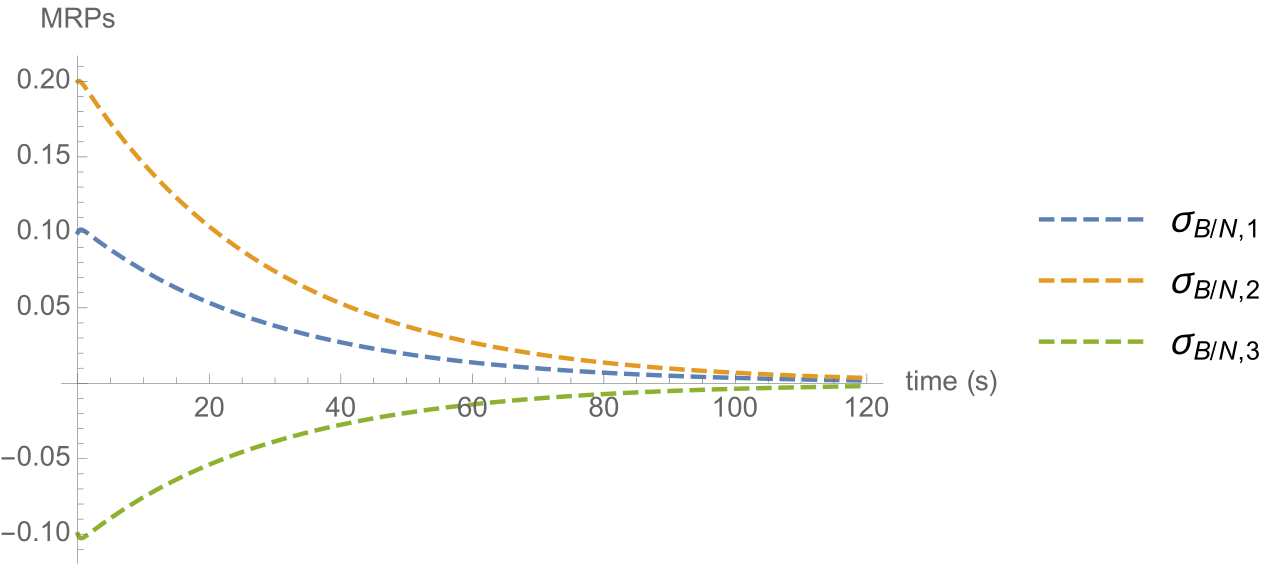
\includegraphics[scale=0.3]{figs/fig_mrp_response_1.png}
\captionsetup{labelformat=empty}
\label{fig_mrp_response_1}
\end{figure}

\begin{figure}[ht]
\centering
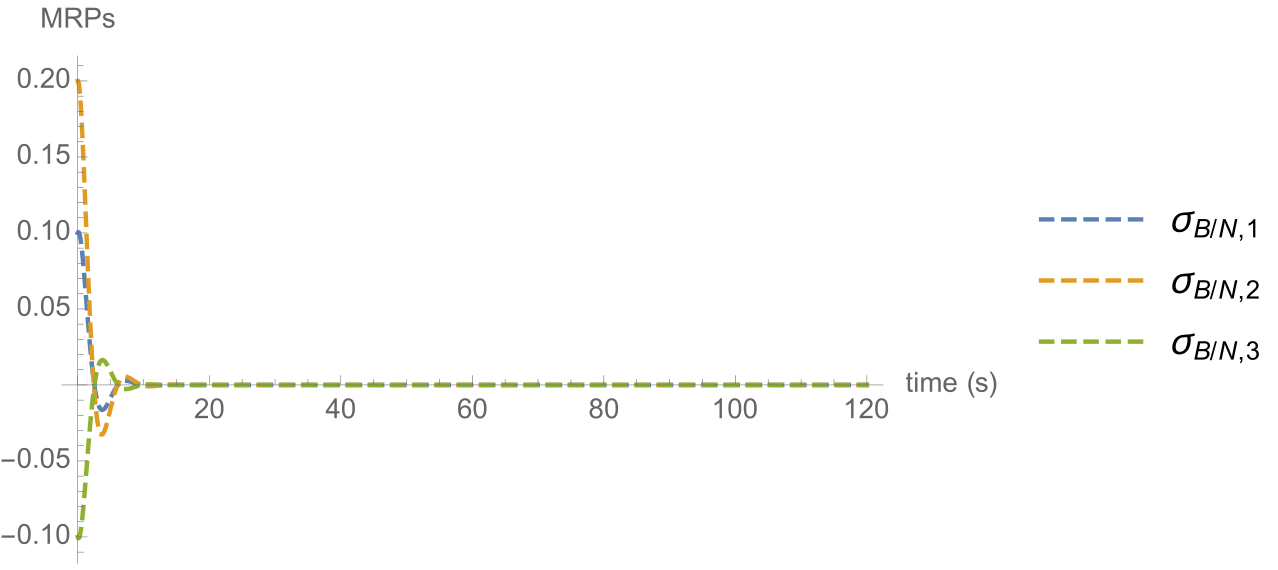
\includegraphics[scale=0.3]{figs/fig_mrp_response_2.png}
\captionsetup{labelformat=empty}
\label{fig_mrp_response_2}
\end{figure}

\begin{figure}[ht]
\centering
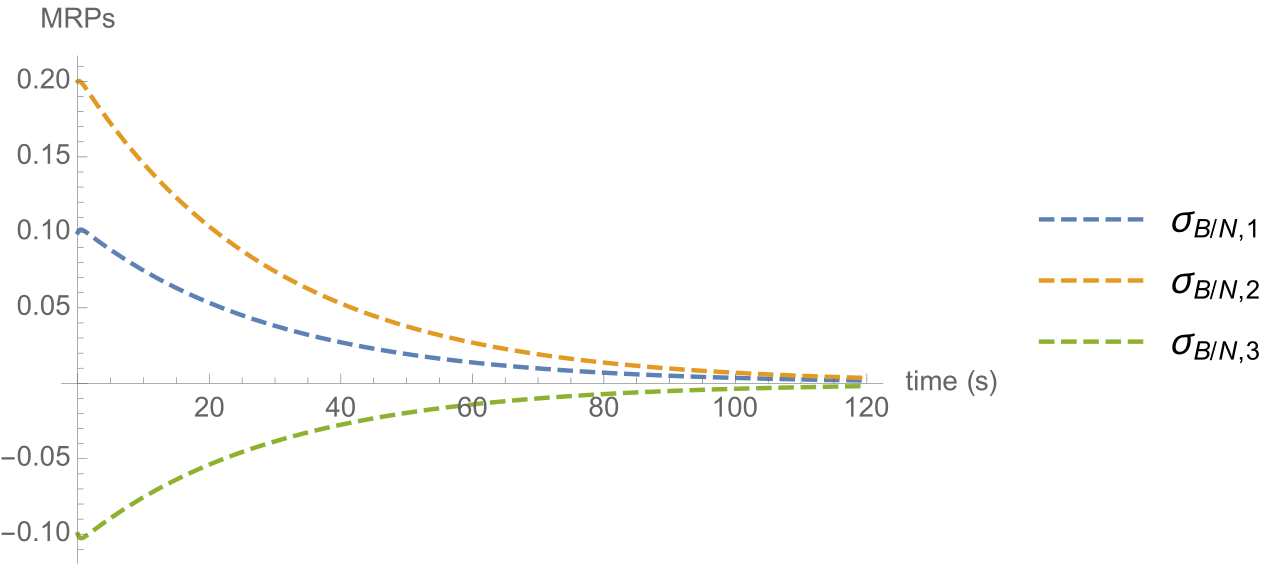
\includegraphics[scale=0.3]{figs/fig_mrp_response_1.png}
\captionsetup{labelformat=empty}
\label{fig_mrp_response_3}
\end{figure}

\paragraph{3.}
Next, simulate this control law $\bm{u}$ with $\bm{\omega}_{\mathcal{B}/\mathcal{N}}(t_{o}) = (30, 10, -20)$ and illustrate the resulting attitude motion using MRPs. What is the tracking error MRP norm $|\bm{\sigma}_{\mathcal{B}/\mathcal{R}}|$ at 50 seconds into the simulation?
\paragraph{\textcolor{orange}{Solution}}0.046204

\newpage
\subsection{RW Feedback Control}

\paragraph{1.}
Assume a spacecraft has 3 RWs attached with $\hat{\bm{g}}_{s_{1}} = \hat{\bm{g}}_{s_{2}} = \hat{\bm{g}}_{s_{3}}$. In this case, for a general control torque $\bm{L}_{r}$, can suitable motor torques $u_{s_{i}}$ always be found?

\begin{itemize}
\noans Yes, the $[\bm{G}_{s}]$ is a $3\times3$ matrix and thus always invertible
\noans Yes, with three wheels you can create any general control torque
\ans No, the three $\hat{\bm{g}}_{s_{i}}$ control axis only span a 1-dimensional space, and thus cannot produce a general $\bm{L}_{r}$ control vector
\end{itemize}

\paragraph{2.}
Assume a spacecraft has 3 RWs attached with $\hat{\bm{g}}_{s_{i}} = \hat{\bm{b}}_{i}$ and $\hat{\bm{b}}_{i}$ are the frame base vectors. What is a benefit of this configuration?

\begin{itemize}
    \noans This configuration is very robust if a wheel fails
    \noans This configuration requires the least amount of power to produce $\bm{L}_{r}$
    \ans This configuration results in $[\bm{G}_{s}]=[\bm{I}_{3\times3}]$ which simplifies the control law formulation
\end{itemize}

\paragraph{3.}
Assume a spacecraft has 4 RWs attached with:
\begin{equation}
\begin{split}
\hat{\bm{g}}_{s_{1}} &= (0.267261,0.534522,0.801784) \\
\hat{\bm{g}}_{s_{2}} &= (-0.267261,0.534522,0.801784) \\
\hat{\bm{g}}_{s_{3}} &= (0.534522,0.267261,0.801784) \\
\hat{\bm{g}}_{s_{4}} &= (-0.666667,0.666667,0.333333) \\
\end{split}
\end{equation}

where the vector components are given with respect to the body frame.  If the control solutions required $ \bm{L}_{r} = (0.1, 0.2, 0.4)$ Nm, what is the smallest set of motor torques $u_{s_{i}}$ that produces this control torque?

\begin{itemize}
\noans $\bm{u}_{s} = (0.062361,0.187083,0.249444)$ Nm
\noans $\bm{u}_{s} = (0.454344,0.400892,0.427618,0.200000)$ Nm
\ans $\bm{u}_{s} = ((0.110482,0.207706,0.194448,-0.0330709)$ Nm
\end{itemize}

\end{document}